%% BioMed_Central_Tex_Template_v1.06
%%                                      %
%  bmc_article.tex            ver: 1.06 %
%                                       %

%%IMPORTANT: do not delete the first line of this template
%%It must be present to enable the BMC Submission system to
%%recognise this template!!

%%%%%%%%%%%%%%%%%%%%%%%%%%%%%%%%%%%%%%%%%
%%                                     %%
%%  LaTeX template for BioMed Central  %%
%%     journal article submissions     %%
%%                                     %%
%%          <8 June 2012>              %%
%%                                     %%
%%                                     %%
%%%%%%%%%%%%%%%%%%%%%%%%%%%%%%%%%%%%%%%%%

%%%%%%%%%%%%%%%%%%%%%%%%%%%%%%%%%%%%%%%%%%%%%%%%%%%%%%%%%%%%%%%%%%%%%
%%                                                                 %%
%% For instructions on how to fill out this Tex template           %%
%% document please refer to Readme.html and the instructions for   %%
%% authors page on the biomed central website                      %%
%% https://www.biomedcentral.com/getpublished                      %%
%%                                                                 %%
%% Please do not use \input{...} to include other tex files.       %%
%% Submit your LaTeX manuscript as one .tex document.              %%
%%                                                                 %%
%% All additional figures and files should be attached             %%
%% separately and not embedded in the \TeX\ document itself.       %%
%%                                                                 %%
%% BioMed Central currently use the MikTex distribution of         %%
%% TeX for Windows) of TeX and LaTeX.  This is available from      %%
%% https://miktex.org/                                             %%
%%                                                                 %%
%%%%%%%%%%%%%%%%%%%%%%%%%%%%%%%%%%%%%%%%%%%%%%%%%%%%%%%%%%%%%%%%%%%%%

%%% additional documentclass options:
%  [doublespacing]
%  [linenumbers]   - put the line numbers on margins

%%% loading packages, author definitions

%\documentclass[twocolumn]{bmcart}% uncomment this for twocolumn layout and comment line below
\documentclass{bmcart}

%%% Load packages
\usepackage{amsthm,amsmath}
%\RequirePackage[numbers]{natbib}
%\RequirePackage[authoryear]{natbib}% uncomment this for author-year bibliography
%\RequirePackage{hyperref}
\usepackage[utf8]{inputenc} %unicode support
%\usepackage[applemac]{inputenc} %applemac support if unicode package fails
%\usepackage[latin1]{inputenc} %UNIX support if unicode package fails

%%%%%%%%%%%%%%%%%%%%%%%%%%%%%%%%%%%%%%%%%%%%%%%%%
%%                                             %%
%%  If you wish to display your graphics for   %%
%%  your own use using includegraphic or       %%
%%  includegraphics, then comment out the      %%
%%  following two lines of code.               %%
%%  NB: These line *must* be included when     %%
%%  submitting to BMC.                         %%
%%  All figure files must be submitted as      %%
%%  separate graphics through the BMC          %%
%%  submission process, not included in the    %%
%%  submitted article.                         %%
%%                                             %%
%%%%%%%%%%%%%%%%%%%%%%%%%%%%%%%%%%%%%%%%%%%%%%%%%
\usepackage{graphicx}
%\def\includegraphic{}
%\def\includegraphics{}

%% add my package
%\usepackage{hyperref}
\usepackage{multirow}
\usepackage{multicol}
\usepackage{makecell}

%%% Put your definitions there:
\startlocaldefs
\endlocaldefs

%%% Begin ...
\begin{document}

%%% Start of article front matter
\begin{frontmatter}

\begin{fmbox}
\dochead{Research}

%%%%%%%%%%%%%%%%%%%%%%%%%%%%%%%%%%%%%%%%%%%%%%
%%                                          %%
%% Enter the title of your article here     %%
%%                                          %%
%%%%%%%%%%%%%%%%%%%%%%%%%%%%%%%%%%%%%%%%%%%%%%

\title{HiTE, an Ensemble Method for High-Precision Transposable Element Annotation}

%%%%%%%%%%%%%%%%%%%%%%%%%%%%%%%%%%%%%%%%%%%%%%
%%                                          %%
%% Enter the authors here                   %%
%%                                          %%
%% Specify information, if available,       %%
%% in the form:                             %%
%%   <key>={<id1>,<id2>}                    %%
%%   <key>=                                 %%
%% Comment or delete the keys which are     %%
%% not used. Repeat \author command as much %%
%% as required.                             %%
%%                                          %%
%%%%%%%%%%%%%%%%%%%%%%%%%%%%%%%%%%%%%%%%%%%%%%

\author[
  addressref={aff1},                   % id's of addresses, e.g. {aff1,aff2}
% noteref={n1},                        % id's of article notes, if any
  email={kanghu@csu.edu.cn}   % email address
]{\inits{K.H.}\fnm{Kang} \snm{Hu}}
\author[
  addressref={aff1},
  corref={aff1},                       % id of corresponding address, if any
  email={jxwang@mail.csu.edu.cn}
]{\inits{JX.W.}\fnm{Jianxin} \snm{Wang}}

%%%%%%%%%%%%%%%%%%%%%%%%%%%%%%%%%%%%%%%%%%%%%%
%%                                          %%
%% Enter the authors' addresses here        %%
%%                                          %%
%% Repeat \address commands as much as      %%
%% required.                                %%
%%                                          %%
%%%%%%%%%%%%%%%%%%%%%%%%%%%%%%%%%%%%%%%%%%%%%%

\address[id=aff1]{%                           % unique id
  \orgdiv{Hunan Provincial Key Lab on Bioinformatics, School of Computer Science and Engineering},             % department, if any
  \orgname{Central South University},          % university, etc
  \city{Changsha, 410083},                              % city
  \cny{China}                                    % country
}

%\address[id=aff2]{%
%  \orgdiv{Institute of Biology},
%  \orgname{National University of Sciences},
%  %\street{},
%  %\postcode{}
%  \city{Kiel},
%  \cny{Germany}
%}

%%%%%%%%%%%%%%%%%%%%%%%%%%%%%%%%%%%%%%%%%%%%%%
%%                                          %%
%% Enter short notes here                   %%
%%                                          %%
%% Short notes will be after addresses      %%
%% on first page.                           %%
%%                                          %%
%%%%%%%%%%%%%%%%%%%%%%%%%%%%%%%%%%%%%%%%%%%%%%

%\begin{artnotes}
%%\note{Sample of title note}     % note to the article
%\note[id=n1]{Equal contributor} % note, connected to author
%\end{artnotes}

\end{fmbox}% comment this for two column layout

%%%%%%%%%%%%%%%%%%%%%%%%%%%%%%%%%%%%%%%%%%%%%%%
%%                                           %%
%% The Abstract begins here                  %%
%%                                           %%
%% Please refer to the Instructions for      %%
%% authors on https://www.biomedcentral.com/ %%
%% and include the section headings          %%
%% accordingly for your article type.        %%
%%                                           %%
%%%%%%%%%%%%%%%%%%%%%%%%%%%%%%%%%%%%%%%%%%%%%%%

\begin{abstractbox}

\begin{abstract} % abstract
\parttitle{Background} %if any
Text for this section.

\parttitle{Results} %if any
Text for this section.

\parttitle{Conclusions} %if any
Text for this section.
\end{abstract}

%%%%%%%%%%%%%%%%%%%%%%%%%%%%%%%%%%%%%%%%%%%%%%
%%                                          %%
%% The keywords begin here                  %%
%%                                          %%
%% Put each keyword in separate \kwd{}.     %%
%%                                          %%
%%%%%%%%%%%%%%%%%%%%%%%%%%%%%%%%%%%%%%%%%%%%%%

\begin{keyword}
\kwd{sample}
\kwd{article}
\kwd{author}
\end{keyword}

% MSC classifications codes, if any
%\begin{keyword}[class=AMS]
%\kwd[Primary ]{}
%\kwd{}
%\kwd[; secondary ]{}
%\end{keyword}

\end{abstractbox}
%
%\end{fmbox}% uncomment this for two column layout

\end{frontmatter}

%%%%%%%%%%%%%%%%%%%%%%%%%%%%%%%%%%%%%%%%%%%%%%%%
%%                                            %%
%% The Main Body begins here                  %%
%%                                            %%
%% Please refer to the instructions for       %%
%% authors on:                                %%
%% https://www.biomedcentral.com/getpublished %%
%% and include the section headings           %%
%% accordingly for your article type.         %%
%%                                            %%
%% See the Results and Discussion section     %%
%% for details on how to create sub-sections  %%
%%                                            %%
%% use \cite{...} to cite references          %%
%%  \cite{koon} and                           %%
%%  \cite{oreg,khar,zvai,xjon,schn,pond}      %%
%%                                            %%
%%%%%%%%%%%%%%%%%%%%%%%%%%%%%%%%%%%%%%%%%%%%%%%%

%%%%%%%%%%%%%%%%%%%%%%%%% start of article main body
% <put your article body there>

%%%%%%%%%%%%%%%%
%% Background %%
%%
\section*{Background}
Text and results for this section, as per the individual journal's instructions for authors.

\begin{figure}[h!]
	\centerline{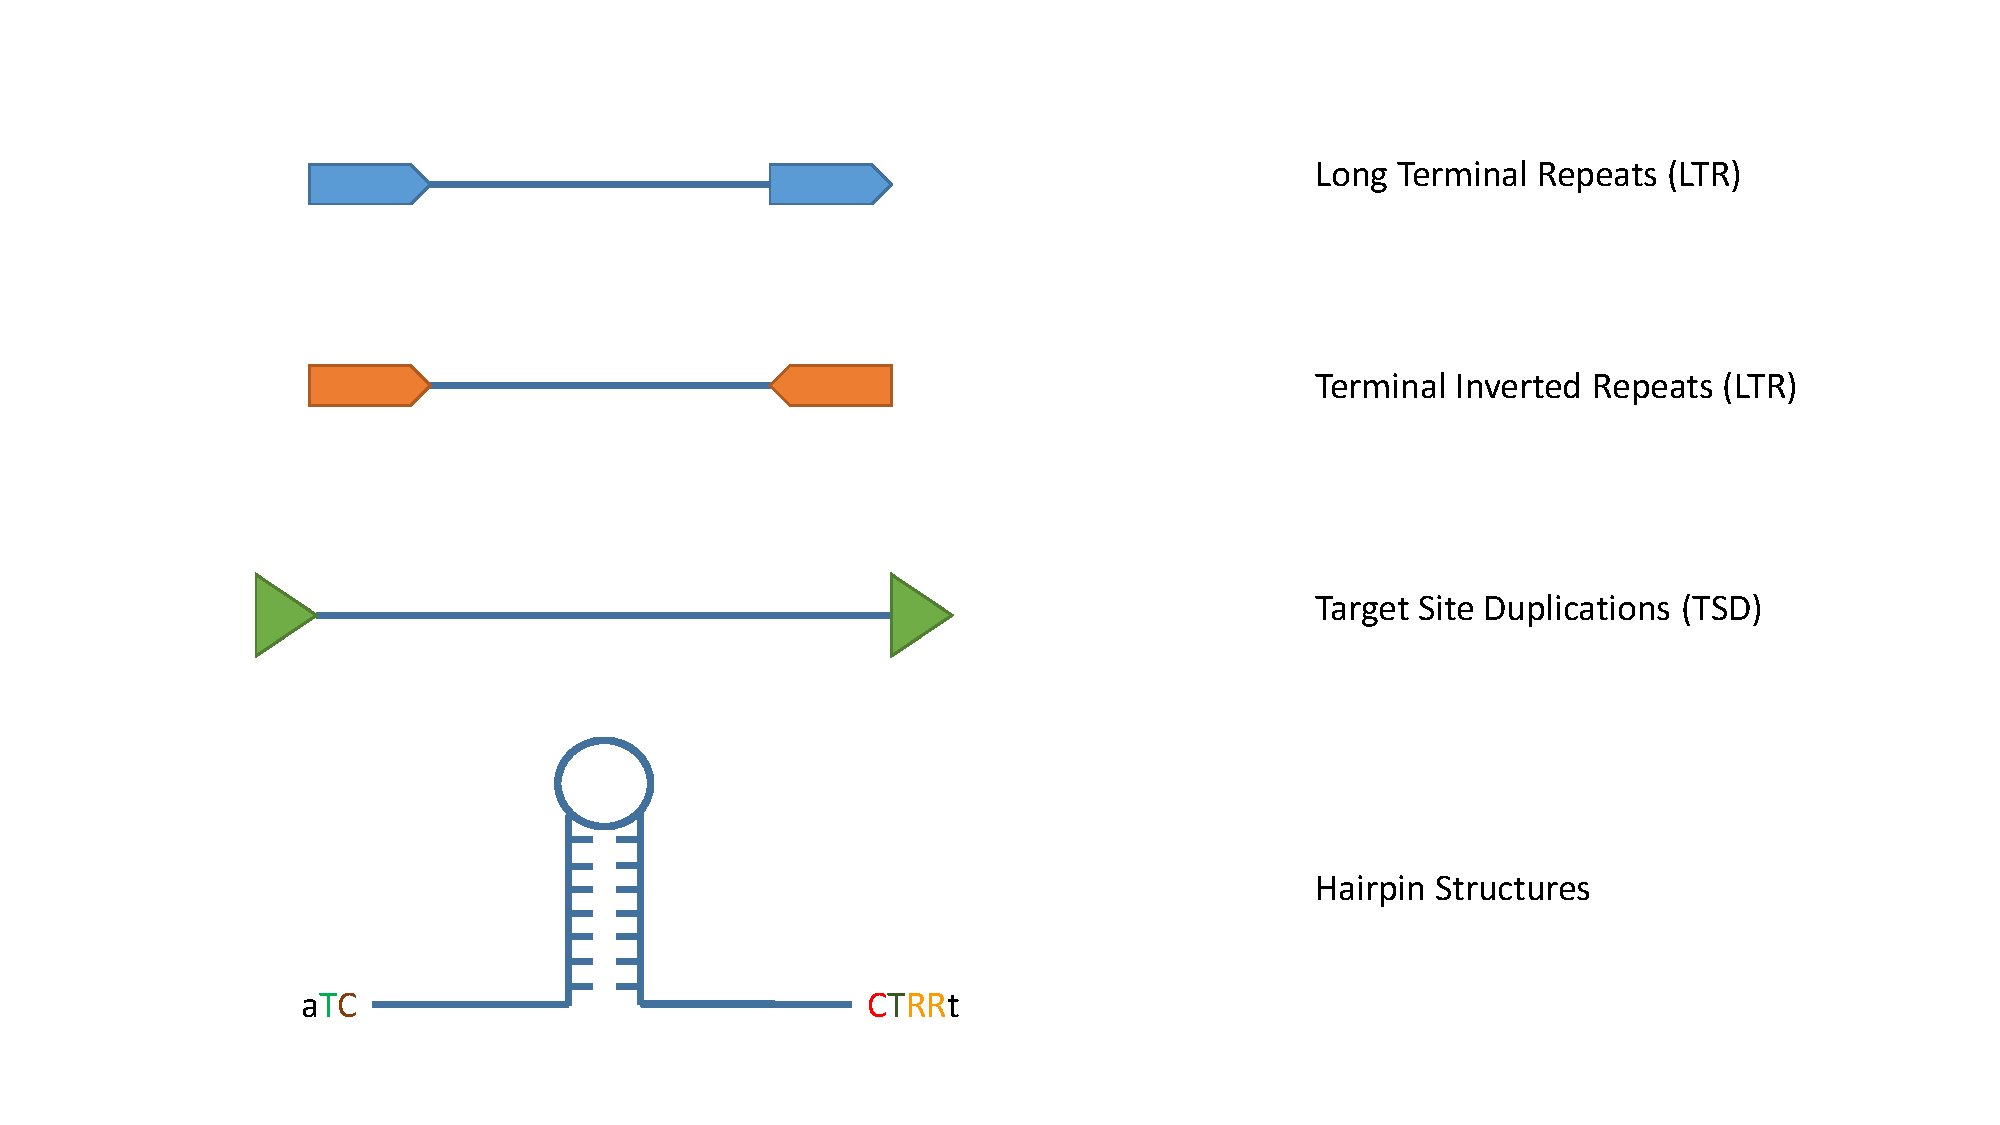
\includegraphics[width=1.0\textwidth]{figures/TEStructures.pdf}}
	\caption{Examples of commonly used TE structural features for detection. The LTR, TIR, TSD, and hairpin structures are used to identify LTR elements, class II elements, and Helitrons, respectively.}
	\label{fig:TE_structures}
\end{figure}

\section*{Results}
In eukaryotic genomes, transposable elements (TEs) exist widely in the form of both full-length (structurally intact) and fragmented sequences. An ideal library should contain only full-length models of all significantly distinct TEs that have left copies in the genome \cite{storer2022methodologies}, which are then used to detect fragmented and divergent TE sequences that are hard to recognize using structural features. However, compared with the limited number of full-length TE sequences, fragmented sequences are more abundant and comprise the majority of TE, creating a challenge for algorithms to find the true ends of the TEs.

The identification methods based on sequence repeatedness tend to produce more fragmented TE sequences, and their sequence boundaries are often approximate, which still need extensive editing before they can be accepted in curated databases such as Dfam or Repbase. For example, the majority of TE models in Dfam come from libraries generated by RepeatModeler, and the great majority of Dfam submissions are currently housed in a non-curated section\cite{storer2021dfam}. Structure-based methods can clearly define the boundaries of the TE structure, but always with a high number of false positives.

To evaluate the performance of different TE identification methods, a high diversity of benchmarking approaches has been proposed, which is a barrier to both the understanding of the true performance of a method and the competitive em of methods. For example, many em methods promote getting the higher copy number of TE, the higher number of models generated, the longer sequences of output, and the higher N50 of the library, which does not take into account the quality of the dataset produced\cite{storer2022methodologies}.

An ideal method of em should be able to consider both the integrity of TE sequences and the false-positive rate of the TE library. To solve this problem, we take the em methods from the latest study, EDTA\cite{ou2019benchmarking} and RepeatModeler2\cite{flynn2020repeatmodeler2}, which could produce ten metrics including \emph{Sensitivity}, \emph{Specificity}, \emph{Accuracy}, \emph{Precision}, \emph{FDR}, \emph{F1}, \emph{Perfect}, \emph{Good}, \emph{Present}, and \emph{Not\_found}. By combining the two complementary em methods, we can accurately evaluate the integrity of TE families and the false-positive rate of the whole TE library.


\subsection*{Selecting benchmarking model species}
Despite the universality and importance of TEs in genomes, except for a few model species, the annotation and research of TEs in other species are still poor. In this benchmarking, we mainly focus on 4 typical species: Oryza sativa, Caenorhabditis briggsae, Drosophila melanogaster, and Danio rerio, whose TE libraries are well studied and preserved. These four species cover genomes of different sizes as well as different TE landscapes. The smallest genome, the C. briggsae genome, is dominated by DNA transposons; the D. melanogaster genome is primarily composed of LTR and LINE transposons; the proportion of LTR and DNA transposons on Oryza sativa was close, along with a medium-sized genome; and the largest genome, the D. rerio genome, comprises the majority of DNA transposons but also some LTR transposons.

Repbase Update (RU) is a database of representative repeat sequences in eukaryotic genomes that has a long history of TE discovery and annotation since 1992\cite{bao2015repbase}. RU has long been used as a manually curated reference database for nearly all eukaryotic genome sequence analyses. Here, we used TE libraries from RepBase26.05 as the gold standard for all species. The RepBase libraries were then used to annotate the genomes for both structurally intact and fragmented TE sequences, which comprised 47.81\% of the O. sativa genome, 15.83\% of the C. briggsae genome, 20.28\% of the D. melanogaster genome, and 57.36\% of the D. rerio genome, respectively (Tables \ref{o.sativa_repbase}, \ref{c.briggsae_repbase}, \ref{d.melanogaster_repbase}, and \ref{d.rerio_repbase}). 

\begin{table}[h!]
	\caption{TE content in the O. sativa (Oryza sativa Japonica Group ``assembly IRGSP-1.0") genome.}\label{o.sativa_repbase}
	\setlength{\tabcolsep}{5.0 mm}{
		\renewcommand{\arraystretch}{1.5}
	\begin{tabular}{ccccc}
		\hline
		& Class & RepBase26.05  & Number of elements & Total (\%)\\ \hline
		LTR & Class I & 88.4 Mb & 46595 & 23.61 \\
		Non-LTR & Class I & 5.7 Mb & 13381 & 1.51 \\
		TIR & Class II  & 67.7 Mb & 230281 & 18.09 \\
		Helitron & Class II & 17.2 Mb & 66469 & 4.60 \\
		Total & - & 179.0 Mb & 356726 & 47.81 \\ \hline
	\end{tabular}
	}
\end{table}

\begin{table}[h!]
	\caption{TE content in the C. briggsae (Caenorhabditis briggsae ``assembly CB4") genome.}\label{c.briggsae_repbase}
	\setlength{\tabcolsep}{5.0 mm}{
		\renewcommand{\arraystretch}{1.5}
	\begin{tabular}{ccccc}
		\hline
		& Class & RepBase26.05  & Number of elements & Total (\%)\\ \hline
		LTR & Class I & 0.2 Mb & 234 & 0.2 \\
		Non-LTR & Class I & 0.9 Mb & 3085 & 0.59 \\
		TIR & Class II  & 14.5 Mb & 68146 & 13.41 \\
		Helitron & Class II & 1.8 Mb & 8509 & 1.63 \\
		Total & - & 17.4 Mb & 79974 & 15.83 \\ \hline
	\end{tabular}}
\end{table}

\begin{table}[h!]
	\caption{TE content in the D. melanogaster (Drosophila melanogaster ``assembly Release 6 plus ISO1 MT") genome.}\label{d.melanogaster_repbase}
	\setlength{\tabcolsep}{5.0 mm}{
		\renewcommand{\arraystretch}{1.5}
	\begin{tabular}{ccccc}
		\hline
		& Class & RepBase26.05  & Number of elements & Total (\%)\\ \hline
		LTR & Class I & 19.9 Mb & 21050 & 11.78 \\
		Non-LTR & Class I & 10.8 Mb & 15428 & 6.37 \\
		TIR & Class II  & 2.6 Mb & 6204 & 1.53 \\
		Helitron & Class II & 1.0 Mb & 4822 & 0.60 \\
		Total & - & 34.2 Mb & 47504 & 20.28 \\ \hline
	\end{tabular}}
\end{table}

\begin{table}[h!]
	\caption{TE content in the D. rerio (Danio rerio ``assembly GRCz11") genome.}\label{d.rerio_repbase}
	\setlength{\tabcolsep}{5.0 mm}{
		\renewcommand{\arraystretch}{1.5}
	\begin{tabular}{ccccc}
		\hline
		& Class & RepBase26.05  & Number of elements & Total (\%)\\ \hline
		LTR & Class I & 119.0 Mb & 296556 & 7.09 \\
		Non-LTR & Class I & 74.3 Mb & 215393 & 4.42 \\
		TIR & Class II  & 719.4 Mb & 3372500 & 42.84 \\
		Helitron & Class II & 50.5 Mb & 178913 & 3.01 \\
		Total & - & 963.2 Mb & 4063362 & 57.36 \\ \hline
	\end{tabular}}
\end{table}

\subsection*{Setting up benchmarking methods for TE library evaluation}
To fairly and comprehensively measure the quality of TE libraries generated by different TE identification tools, we use the benchmarking methods from the latest study, EDTA and RepeatModeler2. For convenience, we hereafter refer to the benchmarking methods of EDTA and RepeatModeler2 as BM\_EDTA and BM\_RM2, respectively. 

As shown in Fig. \ref{fig:benchmarking_methods}A, the BM\_EDTA evaluates the performance of various tools by annotating the genome with the gold standard TE library and the tested TE library generated by these tools. Based on the total number of genomic DNA bases, six metrics, including sensitivity, specificity, accuracy, precision, FDR, and F1, are used to characterize the annotation performance of the tested library\cite{ou2019benchmarking}. The BM\_EDTA can display detailed metrics, including the rates of false positives, which are common in many TE identification methods. However, it cannot reflect the integrity of the TE models. All general repeat identification programs, even those with many fragments and unclear boundaries, still performed well in benchmarking\cite{ou2019benchmarking}. For example, while a 1 kbp intact TE sequence and ten 100 bp fragments may obtain the same performance, the former is obviously more valuable in terms of TE integrity and biological significance.

As shown in Fig. \ref{fig:benchmarking_methods}B, the BM\_RM2 aligns the tested TE library with the gold standard library and divides the gold standard sequences into four levels: ``Perfect", ``Good", ``Present", and ``Not\_found". ``Perfect" families are those for which one sequence in the tested library matches with $>$95\% sequence similarity and $>$95\% length coverage to a family consensus in the gold standard library. ``Good" families are those in which multiple overlapping sequences in the tested library match with $>$95\% similarity and $>$95\% coverage to the curated consensus. A family is considered ``present" if one or multiple library sequences align with $>$80\% similarity and $>$80\% coverage to the reference consensus sequence. Below these thresholds, a family is considered ``not found"\cite{flynn2020repeatmodeler2}. The BM\_RM2 takes the integrity of the sequence into consideration. Intact TE models usually get a perfect level, while fragments can only get a good, present, or even not found level. However, it cannot display the rate of false positives in the tested TE library. By combining the two complementary benchmarking methods, we can accurately evaluate the integrity of TE models and the rate of false positives in the whole TE library.

\begin{figure}[h!]
	\centerline{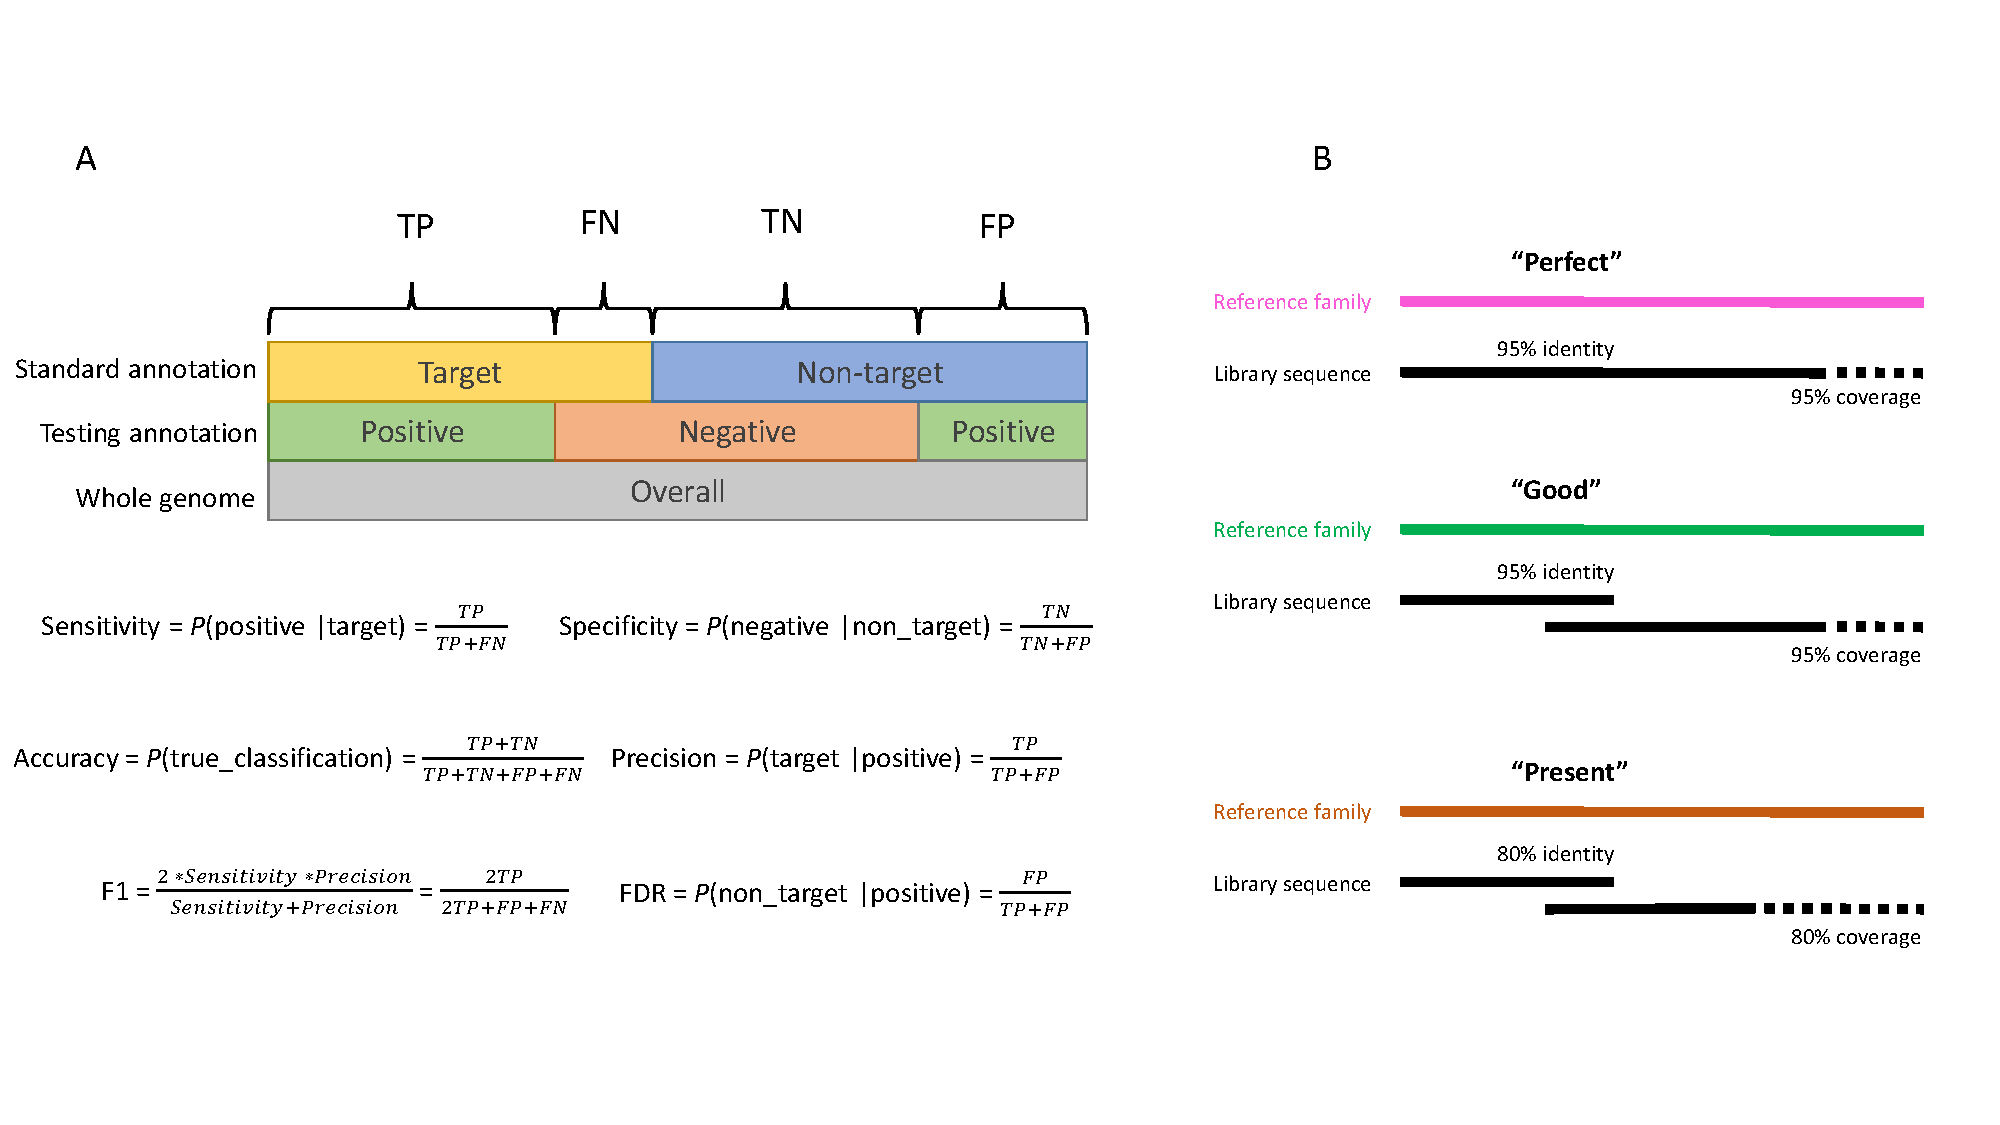
\includegraphics[width=1.0\textwidth]{figures/EvaluationMethods.pdf}}
	\caption{Schematic representation of benchmarking methods. A. EDTA benchmarking methods. B. RepeatModeler2 benchmarking methods.}
	\label{fig:benchmarking_methods}
\end{figure}


\subsection*{Comparison of general-purpose repeat annotators}
We compared HiTE with the other three mainstream general-purpose repeat annotators, including RepeatScout, EDTA, and RepeatModeler2. Among them, EDTA is the best annotation tool based on structure, and RepeatModeler2 is the pipeline with the best overall performance. RepeatScout was originally used to identify repetitive sequences, and its algorithm characteristics tend to find highly consistent repetitive regions, such as duplicates or the youngest TE families. For older and more divergent TEs, many fragments are often generated. RepeatModeler, the old version of RepeatModeler2, uses RECON and RepeatScout for de novo TE identification. Although RECON uses the single linkage clustering algorithm to generate TE sequences based on overlapping alignments, accurate clustering of these alignments is challenging due to the high fragmentation and mosaicism present in TE families\cite{storer2022methodologies}. Therefore, the structurally intact TE models generated by RepeatModeler are not satisfactory (a low number of "perfect" models). To solve this problem, RepeatModeler2 adds the LTR\_retriever module to the RepeatModeler, which generates structurally intact LTR transposons and greatly increase the number of ``Perfect" in the results\cite{flynn2020repeatmodeler2}.

The results of BM\_RM2 are shown in Fig. \ref{fig:total_results}A. Among these methods, we found that RepeatModeler2 is stable on all datasets; the performance of EDTA is unstable, obtaining a high number of perfect models on the TE-rich genomes (Tables \ref{o.sativa_repbase} and \ref{d.rerio_repbase}) but a low number on the other genomes. At the same time, the number of presents is significantly higher than that of other tools, indicating that its results contain many fragments. RepeatScout obtained more perfect sequences on C. briggsae, indicating that the majority of TE in the C. briggsae genome are relatively young, while in other species, it obtained the minimum number of perfect sequences. Since it cannot process more than 1 GB of genomes, it has no results for D. rerio. HiTE has the highest number of perfect TE models than other tools on all datasets and a smaller number of good and present TE models, which shows that HiTE can recognize more structurally intact TE models and fewer fragments; we found that all tools have quite a few ``Not\_Found" TE models, and we discussed in \textbf{Section Discussion}.

The benchmarking results using BM\_EDTA are shown in Fig. \ref{fig:total_results}B. We noticed that RepeatScout and RepeatModeler2 both achieved a consistent high performance, which verified that "all general repeat identification programs, which depend on sequence repeats, performed well" as described in the EDTA\cite{ou2019benchmarking}. The greatest advantage of the BM\_EDTA is that it can intuitively describe the false positive rate of the TE library, but it cannot reflect the integrity of the TE models. For example, in O. sativa and D. melanogaster, RepeatScout has the lowest number of perfect TE models, indicating that there are a large number of fragments, but it has a high BM\_EDTA performance. However, we noticed that on all datasets, HiTE shows significantly higher precision performance, including precision, specificity, and accuracy, which indicates that HiTE can identify TE more accurately. Like the structure-based method EDTA, HiTE achieves a similar low sensitivity, which does not mean that HiTE recognizes fewer TE models than RepeatScout and RepeatModeler2. On the contrary, HiTE obtains more perfect TE models and fewer not\_found TE models from the BM\_RM2 results. 
Since the BM\_EDTA is based on base statistics, some false-positive sequences with short length can be well aligned to the true TEs, resulting in falsely high sensitivity but significantly low precision. Each TE sequence in HiTE has complete structural characteristics and copy verification (at least two full-length copies exist, and the region outside the TE copy boundary has no homology), which leads to high precision and somewhat lower sensitivity.
The reason that RepeatScout and RepeatModeler2 can obtain higher sensitivity is that they identify TE based on the repeatedness of the sequence, so many short and incomplete TE models will also be identified, which are filtered out in HiTE.


\begin{figure}[h!]
	\centerline{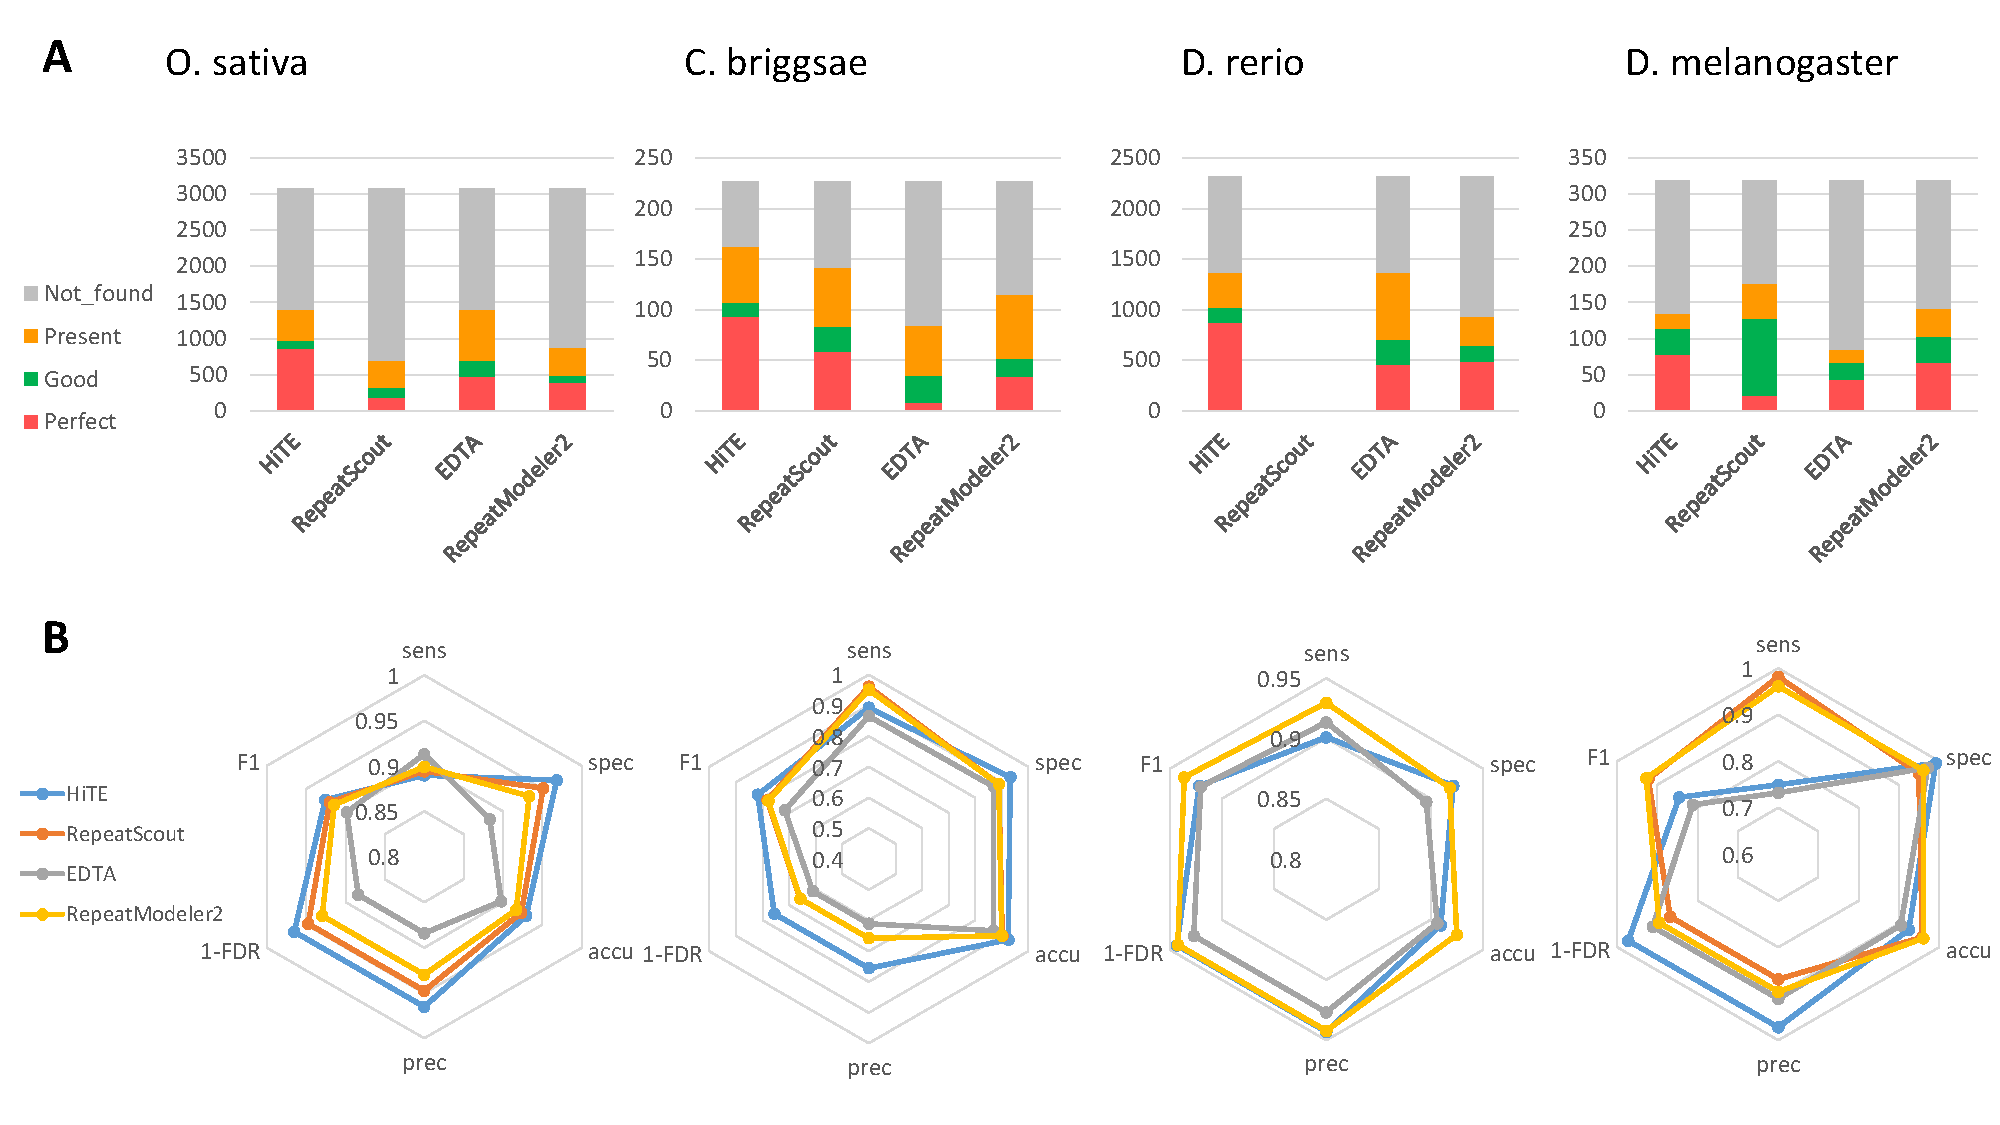
\includegraphics[width=1.0\textwidth]{figures/TotalResults.pdf}}
	\caption{Performance of general-purpose repeat annotators. A the performance based on benckmarking method of RepeatModeler2 and B the performance based on benckmarking method of EDTA.}
	\label{fig:total_results}
\end{figure}

\begin{table}[h!]
	\caption{TE content in the D. rerio (Danio rerio ``assembly GRCz11") genome.}\label{d.rerio_repbase}
	\setlength{\tabcolsep}{5.0 mm}{
		\renewcommand{\arraystretch}{1.5}
		\begin{tabular}{ccccc}
			\hline
			& Class & RepBase26.05  & Number of elements & Total (\%)\\ \hline
			LTR & Class I & 119.0 Mb & 296556 & 7.09 \\
			Non-LTR & Class I & 74.3 Mb & 215393 & 4.42 \\
			TIR & Class II  & 719.4 Mb & 3372500 & 42.84 \\
			Helitron & Class II & 50.5 Mb & 178913 & 3.01 \\
			Total & - & 963.2 Mb & 4063362 & 57.36 \\ \hline
	\end{tabular}}
\end{table}

\begin{table}[h!]
	\caption{Details of performance among general-purpose repeat annotators based on O. sativa.}\label{total_result_rice}
	\setlength{\tabcolsep}{0.15 mm}{
		\renewcommand{\arraystretch}{1.5}
		\begin{tabular}{cccccccccccc}
			\hline
			\multirow{2}{*}{Tools} & \multicolumn{6}{c}{EDTA evaluation} & & \multicolumn{4}{c}{RepeatModeler2 evaluation} \\
			\cline{2-7} \cline{9-12} 
			& Sensitivity & Specificity & Accuracy & Precision & FDR & F1 &  & Perfect & Good & Present & Not\_found \\
			\hline
			HiTE & 0.8897 & 0.9686 & 0.9295 & 0.9653 & 0.0347 & 0.9260 & & 858 & 106 & 430 & 1690 \\
			RepeatScout & 0.8940 & 0.9514 & 0.9230 & 0.9476 & 0.0524 & 0.9200 & & 173 & 149 & 375 & 2387  \\
			EDTA & 0.9131 & 0.8831 & 0.8979 & 0.8840 & 0.1160 & 0.8983 & & 464 & 225 & 709 & 1686 \\
			RepeatModeler2 & 0.8993 & 0.9336 & 0.9166 & 0.9299 & 0.0701 & 0.9144 & & 385 & 94 & 394 & 2211 \\ 
			\hline
	\end{tabular} }
\end{table}

\begin{table}[h!]
	\caption{Details of performance among general-purpose repeat annotators based on C. briggsae.}\label{total_result_cb}
	\setlength{\tabcolsep}{0.15 mm}{
		\renewcommand{\arraystretch}{1.5}
		\begin{tabular}{cccccccccccc}
			\hline
			\multirow{2}{*}{Tools} & \multicolumn{6}{c}{EDTA evaluation} & & \multicolumn{4}{c}{RepeatModeler2 evaluation} \\
			\cline{2-7} \cline{9-12} 
			& Sensitivity & Specificity & Accuracy & Precision & FDR & F1 &  & Perfect & Good & Present & Not\_found \\
			\hline
			HiTE & 0.8926 & 0.9323 & 0.9247 & 0.7550 & 0.2450 & 0.8181 & & 93 & 14 & 55 & 65 \\
			RepeatScout & 0.9616 & 0.8875 & 0.9011 & 0.6583 & 0.3417 & 0.7815 & & 58 & 25 & 59 & 85 \\
			EDTA & 0.8656 & 0.8690 & 0.8683 & 0.6115 & 0.3885 & 0.7167 & & 8 & 27 & 49 & 143 \\
			RepeatModeler2 & 0.9519 & 0.8876 & 0.8995 & 0.6576 & 0.3424 & 0.7778 & & 34 & 17 & 64 & 112 \\ 
			\hline
	\end{tabular} }
\end{table}

\begin{table}[h!]
	\caption{Details of performance among general-purpose repeat annotators based on D. rerio.}\label{total_result_zebrafish}
	\setlength{\tabcolsep}{0.15 mm}{
		\renewcommand{\arraystretch}{1.5}
		\begin{tabular}{cccccccccccc}
			\hline
			\multirow{2}{*}{Tools} & \multicolumn{6}{c}{EDTA evaluation} & & \multicolumn{4}{c}{RepeatModeler2 evaluation} \\
			\cline{2-7} \cline{9-12} 
			& Sensitivity & Specificity & Accuracy & Precision & FDR & F1 &  & Perfect & Good & Present & Not\_found \\
			\hline
			HiTE & 0.9012 & 0.9213 & 0.9094 & 0.9430 & 0.0570 & 0.9216 & & 868 & 147 & 347 & 960 \\
			RepeatScout & - & - & - & - & - & - & & - & - & - & -  \\
			EDTA & 0.9134 & 0.8955 & 0.9061 & 0.9268 & 0.0732 & 0.9201 & & 453 & 252 & 659 & 958  \\
			RepeatModeler2 & 0.9297 & 0.9180 & 0.9249 & 0.9421 & 0.0579 & 0.9359 & & 480 & 159 & 294 & 1389 \\ 
			\hline
	\end{tabular} }
\end{table}

\begin{table}[h!]
	\caption{Details of performance among general-purpose repeat annotators based on D. melanogaster.}\label{total_result_dmel}
	\setlength{\tabcolsep}{0.15 mm}{
		\renewcommand{\arraystretch}{1.5}
		\begin{tabular}{cccccccccccc}
			\hline
			\multirow{2}{*}{Tools} & \multicolumn{6}{c}{EDTA evaluation} & & \multicolumn{4}{c}{RepeatModeler2 evaluation} \\
			\cline{2-7} \cline{9-12} 
			& Sensitivity & Specificity & Accuracy & Precision & FDR & F1 &  & Perfect & Good & Present & Not\_found \\
			\hline
			HiTE & 0.7491 & 0.9917 & 0.9243 & 0.9718 & 0.0282 & 0.8461 & & 77 & 36 & 21 & 186 \\
			RepeatScout & 0.9824 & 0.9493 & 0.9577 & 0.8685 & 0.1315 & 0.9220 & & 21 & 106 & 49 & 144 \\
			EDTA & 0.7322 & 0.9721 & 0.9046 & 0.9113 & 0.0887 & 0.8120 & & 43 & 23 & 19 & 235 \\
			RepeatModeler2 & 0.9614 & 0.9613 & 0.9613 & 0.8956 & 0.1044 & 0.9273 & & 66 & 36 & 39 & 179 \\  
			\hline
	\end{tabular} }
\end{table}

\subsection*{Comparison of TIR annotators}
TIR TEs, which belong to class II TEs, are ancient TEs found in almost all eukaryotes. They are flanked by characteristic terminal inverted repeat sequences (TIRs), usually presenting in low to moderate numbers\cite{wicker2007unified}. TIR TEs may contribute to genome evolution by generating allelic diversity, inducing structural variation, and regulating gene expression\cite{su2019tir}. TIR TEs are divided into nine known superfamilies by the distinguished TIR sequences and the TSD size (usually 2–11 bp). However, due to the short terminal inverted repeat sequences, TIR TE identification and annotation are quite challenging. For example, members of the hAT superfamily have TSDs of 8 bp and relatively short TIRs of 5–27 bp\cite{kempken2001hat}.

Many tools have been designed for their identification, such as IRF\cite{warburton2004inverted}, TIRvish\cite{gremme2013genometools}, TIR-Learner\cite{su2019tir}, and GRF\cite{shi2019generic}, which identify TIR elements by structural signals and are comprehensively evaluated in EDTA. Unfortunately, due to the short structural characteristics of TIR, these methods discover a high number of false positives. For example, the IRF and GRF-TIR produce a large number of candidates, with 4.7 GB and 630 GB (13x–1684x the size of the 374 MB rice genome, respectively) of raw TIR candidate sequences. Among these tools, the TIR module (GRF and TIR-learner) of EDTA has demonstrated great promise for structural annotation and achieved higher performance than other tools\cite{ou2019benchmarking}. However, it is far from high-precision TIR identification. To solve this problem, we developed a new method to achieve high-precision TIR TE identification (see the ``Methods" section).

As shown in Fig. \ref{fig:tir_results}, according to the benchmarking results of the BM\_RM2, our method can identify more perfect TE models, while the number of good and present models is lower. According to the benchmarking results of the BM\_EDTA, our method has higher sensitivity, specificity, accuracy, precision, F1, and a lower FDR than EDTA. These two benchmarking methods both demonstrate that our method can achieve high-precision identification of TIR TEs.

\begin{figure}[h!]
	\centerline{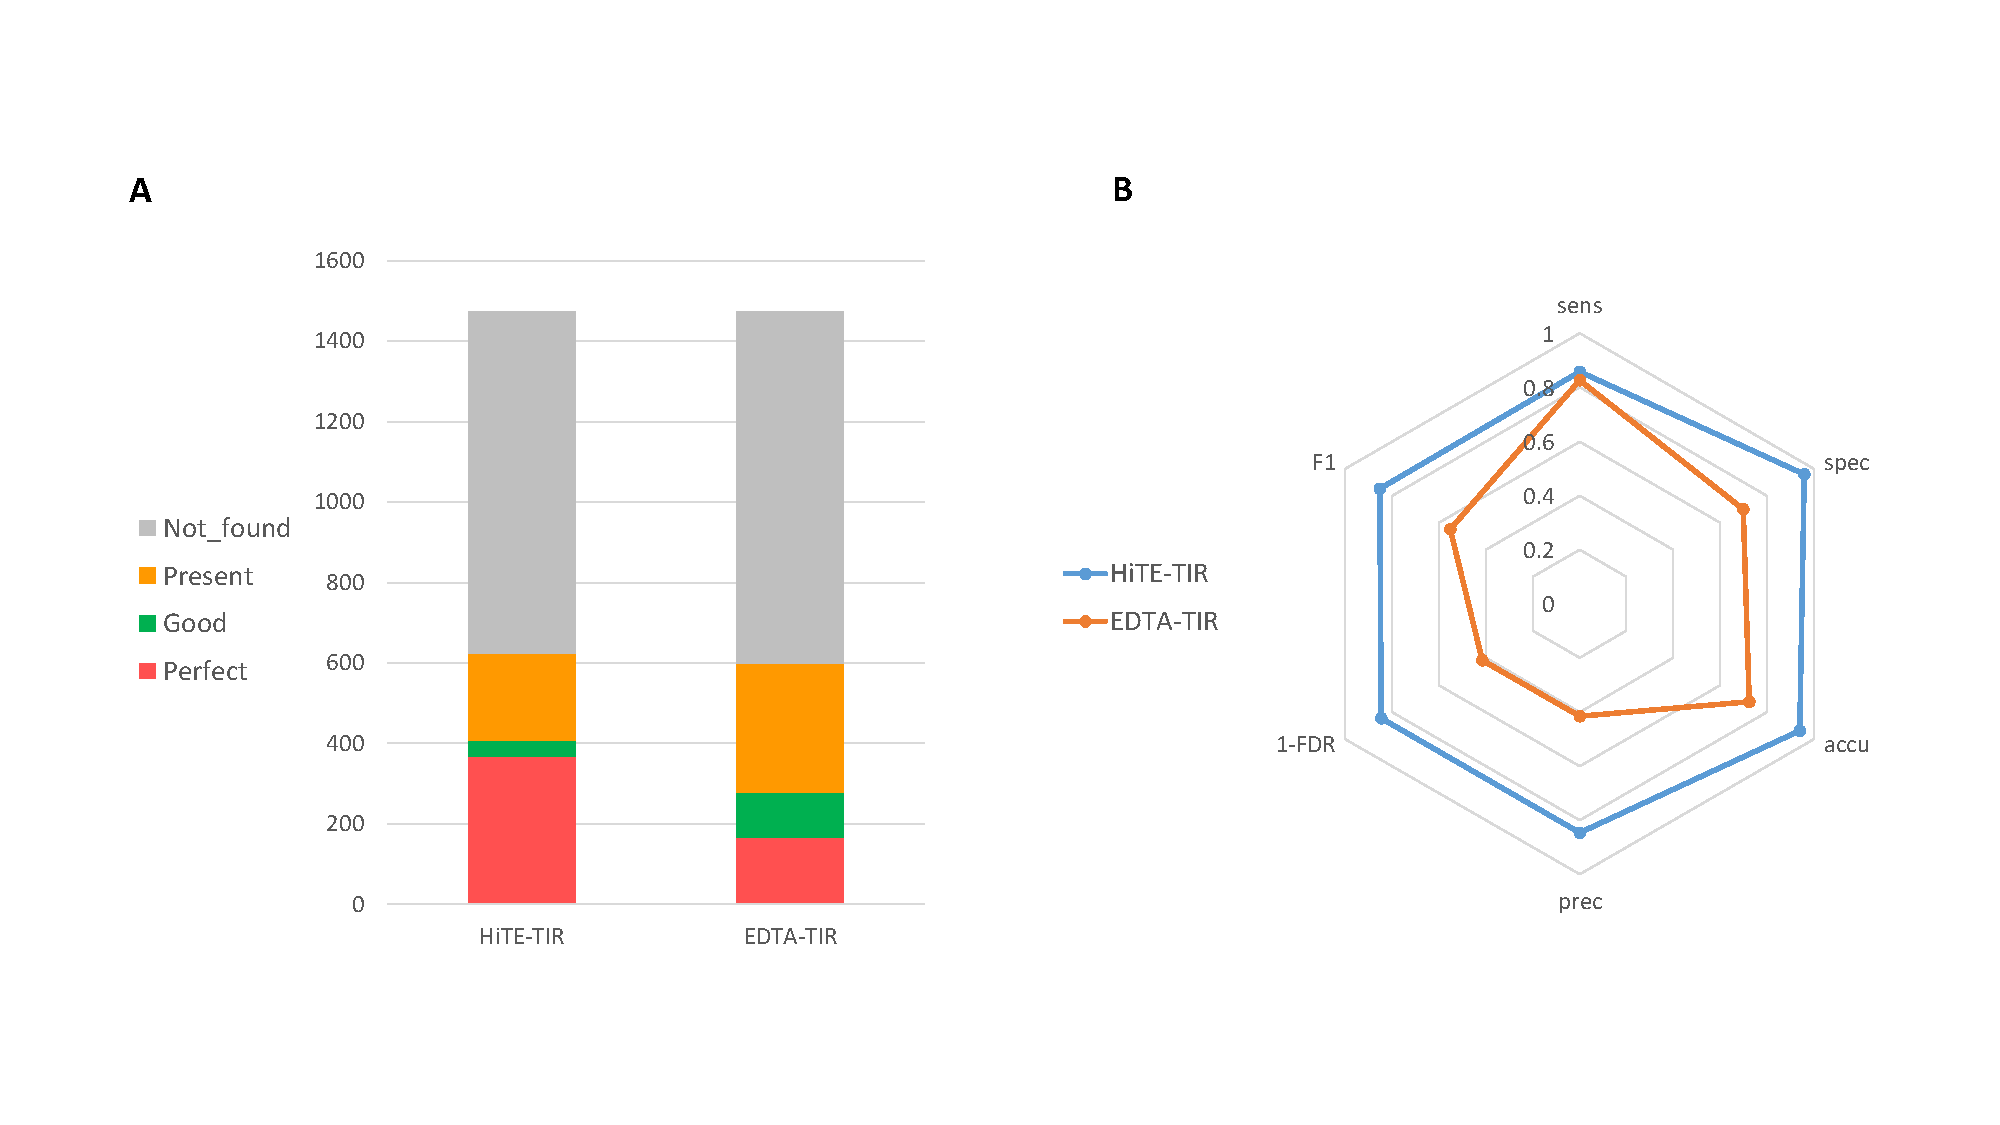
\includegraphics[width=1.0\textwidth]{figures/TIRResults.pdf}}
	\caption{Performance of TIR annotators. A the performance based on benckmarking method of RepeatModeler2 and B the performance based on benckmarking method of EDTA.}
	\label{fig:tir_results}
\end{figure}

\begin{table}[h!]
	\caption{Details of performance among all types of TE annotators based on O. sativa.}\label{all_TE_result_rice}
	\setlength{\tabcolsep}{0.1 mm}{
		\renewcommand{\arraystretch}{1.5}
		\begin{tabular}{cccccccccccccc}
			\hline
			\multirow{2}{*}{TE class} & \multirow{2}{*}{Tools} & \multicolumn{6}{c}{EDTA evaluation} & & \multicolumn{4}{c}{RepeatModeler2 evaluation} \\
			\cline{4-9} \cline{11-14} 
			& & & Sens & Spec & Accu & Prec & FDR & F1 &  & Perfect & Good & Present & Not\_found \\
			\hline
			\multirow{2}{*}{TIR} & EDTA-TIR & & 0.8274 & 0.6989 & 0.7253 & 0.4149 & 0.5851 & 0.5526 & & 165 & 112 & 320 & 877  \\
			& HiTE-TIR & & 0.8607 & 0.9591 & 0.9391 & 0.8431 & 0.1569 & 0.8518 & &  374 & 39 & 217 & 844 \\
			\cline{2-14}
			\multirow{3}{*}{Helitron} & EAHelitron & & 0.2666 & 0.9983 & 0.9135 & 0.9536 & 0.0464 & 0.4167 & & 0 & 0 & 0 & 310   \\
			& \makecell{EDTA-\\HelitronScanner} & & 0.8930 & 0.6259 & 0.6509 & 0.1982 & 0.8018 & 0.3244 & & 4 & 30 & 54 & 222 \\
			& HiTE-Helitron & & 0.7040 & 0.9703 & 0.9438 & 0.7240 & 0.2761 & 0.7138 & & 35 & 14 & 21 & 240  \\
			\cline{2-14}
			\multirow{3}{*}{LTR} & LTRharvest & & 0.9420 & 0.8269 & 0.8548 & 0.6356 & 0.3644 & 0.7590 & & 395 & 56 & 105 & 549  \\
			& LTR\_FINDER & & 0.9676 & 0.8601 & 0.8860 & 0.6874 & 0.3126 & 0.8038 & & 493 & 68 & 117 & 427 \\
			& LTR\_retriever & & 0.9604 & 0.9456 & 0.9491 & 0.8491 & 0.1509 & 0.9013 & & 417 & 46 & 172 & 470  \\
			\cline{2-14}
			\multirow{2}{*}{Non-LTR} & Non\_LTR\_library & & 0.7302 & 0.9879 & 0.9819 & 0.5883 & 0.4117 & 0.6516 & & 77 & 3 & 21 & 48  \\
			& HiTE-Non-LTR & & 0.6519 & 0.9999 & 0.9916 & 0.9906 & 0.0094 & 0.7863 & &  24 & 0 & 21 & 104 \\
			\hline
	\end{tabular} }
\end{table}



We have observed that some new TIR elements have been found, which differ significantly from those in Repbase and are distinguished by the 80\% principle\cite{wicker2007unified}. Through careful inspection, we found that these new TIR elements have a complete TIR and TSD structure, and the boundaries between their copies are clear. Notably, most of them have low copy numbers (Fig. \ref{fig:novel_tirs}). At the same time, nearly half of the sequences in the new DNA TIRs have more than 3 copies (Fig. \ref{fig:novel_tirs}), suggesting that these are like real TEs that were not included in the Repbase library due to their low number of copies.
In addition, we recognize that some TIR TEs have TIRs similar to the known TIRs in Repbase (Fig. \ref{fig:novel_tirs}), which are likely to be non-autonomous TIR TEs.

\begin{figure}[h!]
	\centerline{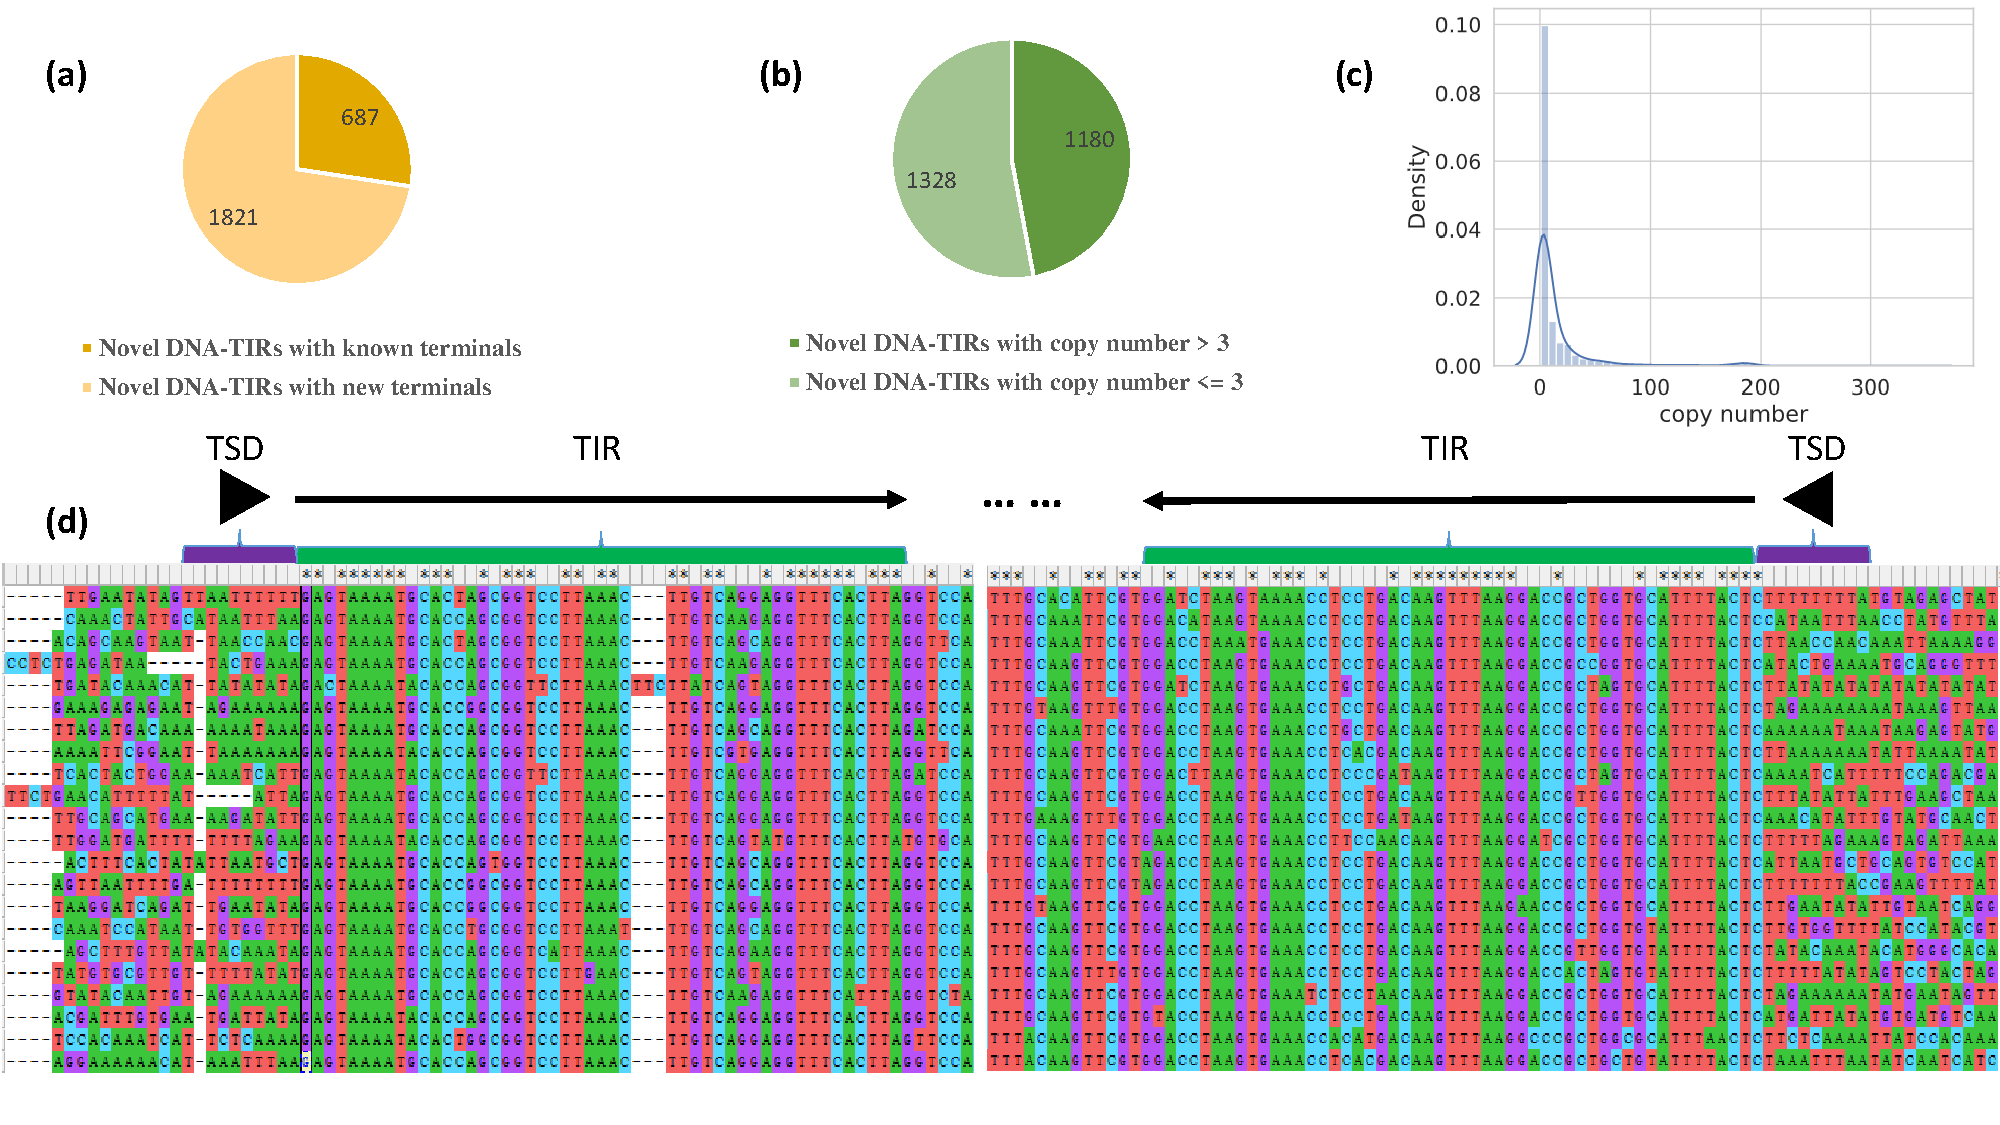
\includegraphics[width=1.0\textwidth]{figures/NovelTIRs.pdf}}
	\caption{Characteristic of novel TIR elements identified by HiTE. A the number of novel TIR elements with different types of terminals; B the ratio of copy numbers $>$ 3 and $<=$ 3; and C the distribution of copy numbers of TIR elements identified by HiTE.}
	\label{fig:novel_tirs}
\end{figure}

\subsection*{Comparison of Helitron annotators}
Helitrons are a subclass of DNA transposons, which replicate through the rolling circle mechanism. When replicating themselves, only the single strand of DNA is broken, and no TSD is generated, which is different from the other TEs. The Helitron transposon has a 5'-TC...-CTRR-3' conserved structure, where R refers to purine, A or G, and there is a short hairpin structure about 10 bp upstream of the 3' end. Helitrons mostly transition into host AT target sites, resulting in flanking 5'-A and 3'-T nucleus\cite{kapitonov2007helitrons}. The weak structural signals of Helitrons make identification of these elements particularly challenging.

To date, there are only two tools, HelitronScanner and EAHelitron, that can produce useful Helitron predictions. HelitronScanner\cite{xiong2014helitronscanner} identifies the sequence patterns in Helitron transposons using the local combinational variable (LCV) algorithm, which produced a large number of candidate sequences, most of which are false positives. For example, 52 MB of raw candidate sequences cover 13.9\% of the rice genome, which obviously exceeds the real coverage. EDTA filters the results of HelitronScanner, greatly improving its specificity and accuracy without reducing its sensitivity\cite{ou2019benchmarking}. Nevertheless, the precision of the Helitron identification module of EDTA is still very low (Fig), which is far from satisfactory.

We also test the other tool, EAHelitron, which identifies Helitrons based on the conservative structure traits using regular expression (RE), such as the 5’ terminal with TC, the 3’ terminal with CTAGt, and a GC-rich hairpin loop before 2–10 nt of CTAG. The performance of EAHelitron is primarily determined by the pre-defined patterns of hairpin loop regular expressions. We observed that it lost some of the hairpin loop patterns of real Helitrons. For example, many real Helitrons in C. briggsae cannot be discovered until we manually add a new pattern of haripin loop ``[GC]{4}". EAHelitron specifies a ``-u" parameter to search all possible 5'-TC upstream of CTAGt-3', and it is hard to know the real 5' end of Helitron. We take the first 5'-TC closest to CTAGt-3' as the 5' end of candidate Helitrons, which leads to extremely short sequences with only 87 bp average length and 44 candidates in rice. The short candidate sequences produce the highest precision but the lowest sensitivity (Fig. \ref{fig:helitron_results}B). Moreover, it cannot identify any gold standard models according to the BM\_RM2 (Fig. \ref{fig:helitron_results}A).

To discover the intact Helitron elements, we have developed a new Helitron identification method, which is a further usage of the coarse boundary TE candidates output by the FMEA algorithm. EAHelitron is used to locate the accurate 3'-CTRR and the hairpin loop structure in candidate TE sequences. The 5'-TC closest to the coarse boundary is selected as the true end. To control the false discovery of the candidate Helitrons, we filtered out the candidates that were not inserted into AT target sites. Finally, the TE copy-based filtering method for region homology outside the boundaries is used to obtain confident candidates (see the ``Methods" section).

The experimental results show that our Helitron identification method has the highest performance (Fig. \ref{fig:helitron_results}), which is superior to EDTA with significantly higher precision, specificity, and accuracy. Compared with the pure EAHelitron method, we have greatly improved the sensitivity and F1 value. We infer that our sensitivity would be greatly improved once EAHelitron can include a more comprehensive hairpin loop pattern. At the same time, we identify more perfect Helitrons in the gold standard dataset. However, we do notice that our results are still affected by false positives, which indicates that our method has potential for improvement.

\begin{figure}[h!]
	\centerline{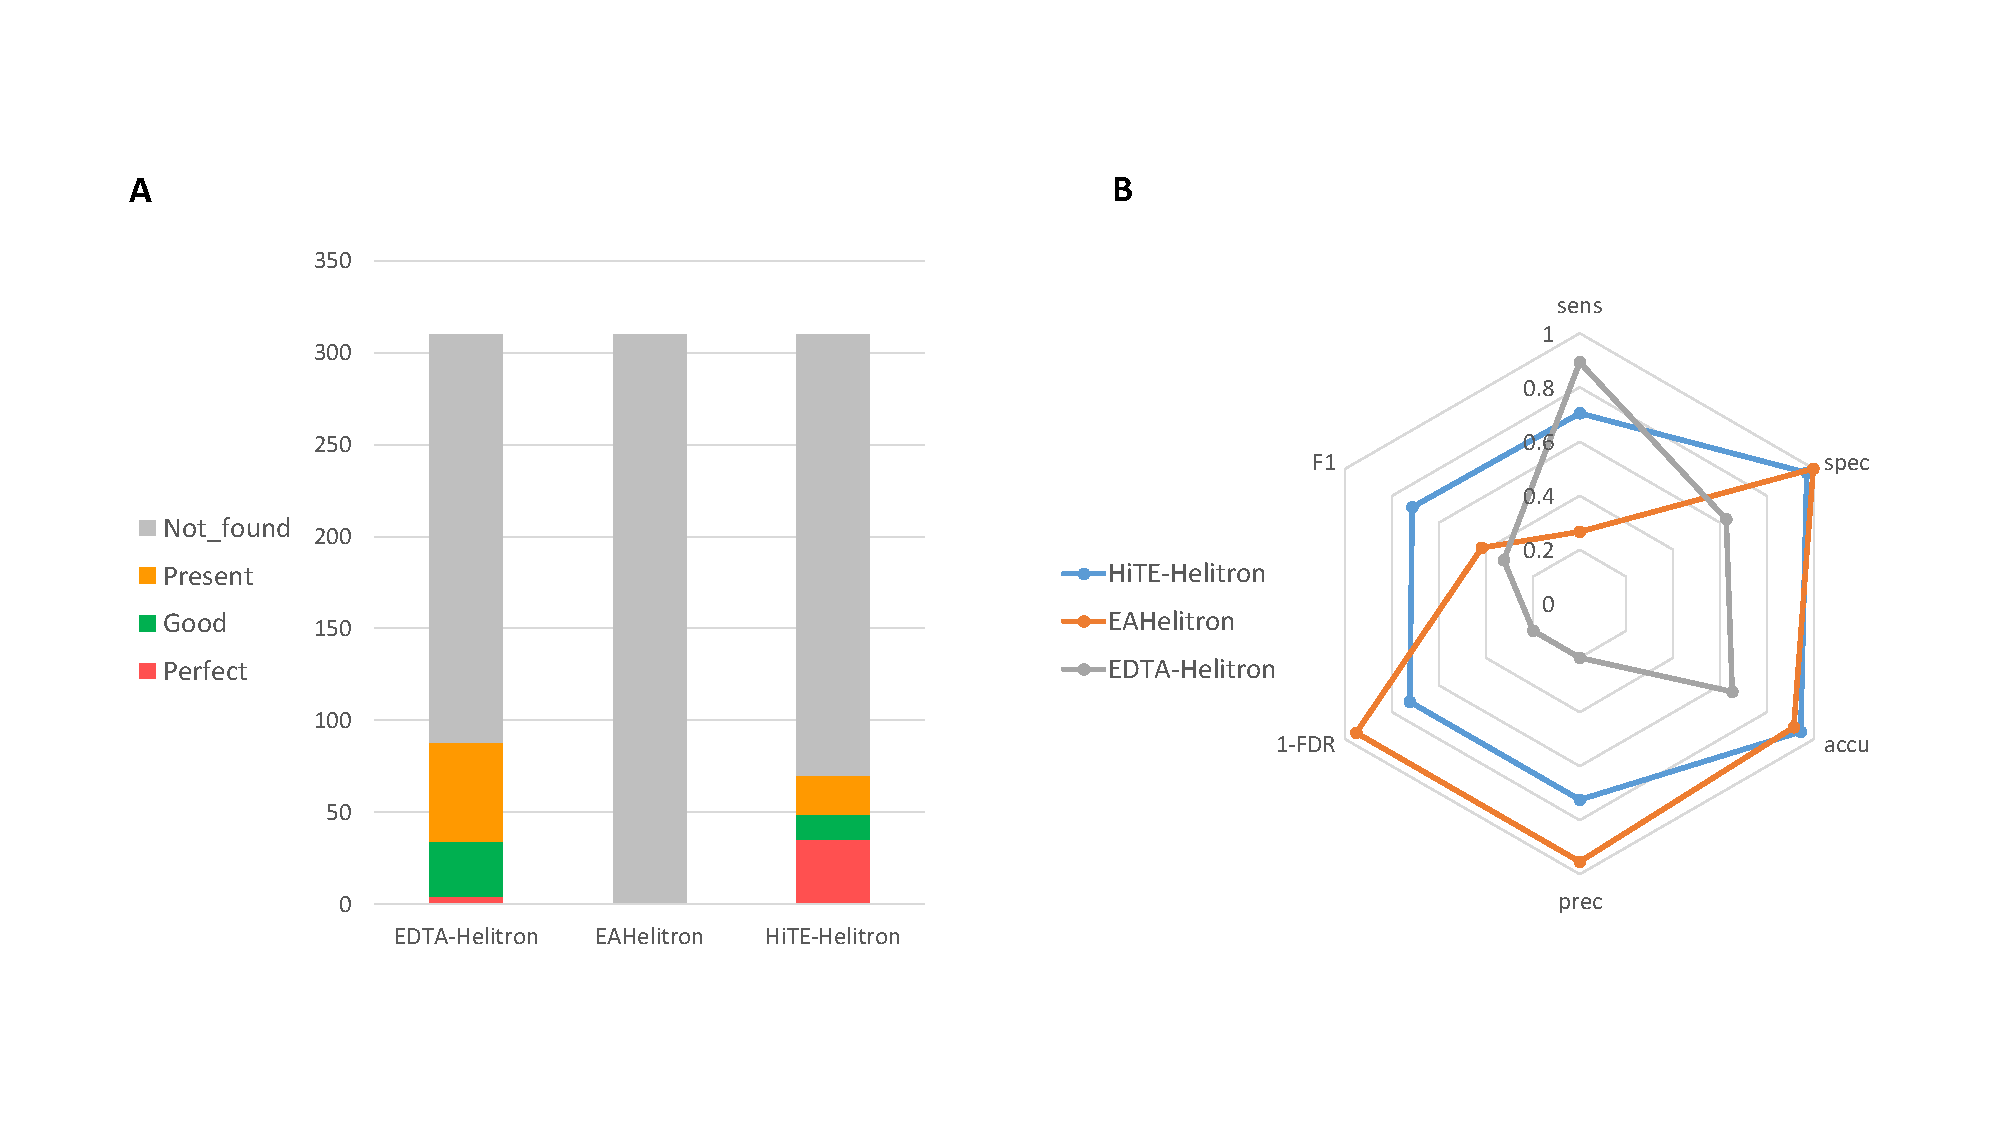
\includegraphics[width=1.0\textwidth]{figures/HelitronResults.pdf}}
	\caption{Performance of Helitron annotators. A the performance based on benckmarking method of RepeatModeler2 and B the performance based on benckmarking method of EDTA.}
	\label{fig:helitron_results}
\end{figure}


\subsection*{Comparison of LTR annotators}
Long terminal repeat retrotransposons (LTR-RTs) (Fig. \ref{fig:ltr_results}) have a well-conserved structure and are prevalent in plant genomes. There are many tools dedicated to the de novo identification of LTR-RTs, including MGEScan3\cite{lee2016mgescan}, GRF, LTR\_STRUC\cite{mccarthy2003ltr_struc}, LTR\_FINDER\cite{xu2007ltr_finder}, LTRharvest\cite{ellinghaus2008ltrharvest}, LtrDetector\cite{valencia2019ltrdetector}, and LTR\_retriever\cite{ou2018ltr_retriever}. It is worth noting that LTR\_retriever was designed as a stringent filtering method for raw results from other LTR tools and does not have its own search engine. We benchmarked the three best existing LTR de novo identification tools, LTR\_FINDER, LTRharvest and LTR\_retriever (using the output of LTR\_FINDER and LTRharvest as input), and found that LTR\_FINDER and LTRharvest achieve higher sensitivity but lower precision, whereas LTR\_retriever significantly improves the precision while maintaining the same sensitivity. The LTR\_retriever was integrated into a variety of TE detection pipelines, including EDTA and RepeatModeler2, and greatly improved the accuracy of their LTR identification. Although LTR\_retriever loses some perfect models, it is still the best LTR identification method at present. Therefore, we integrated LTR\_retriever into HiTE.

\begin{figure}[h!]
	\centerline{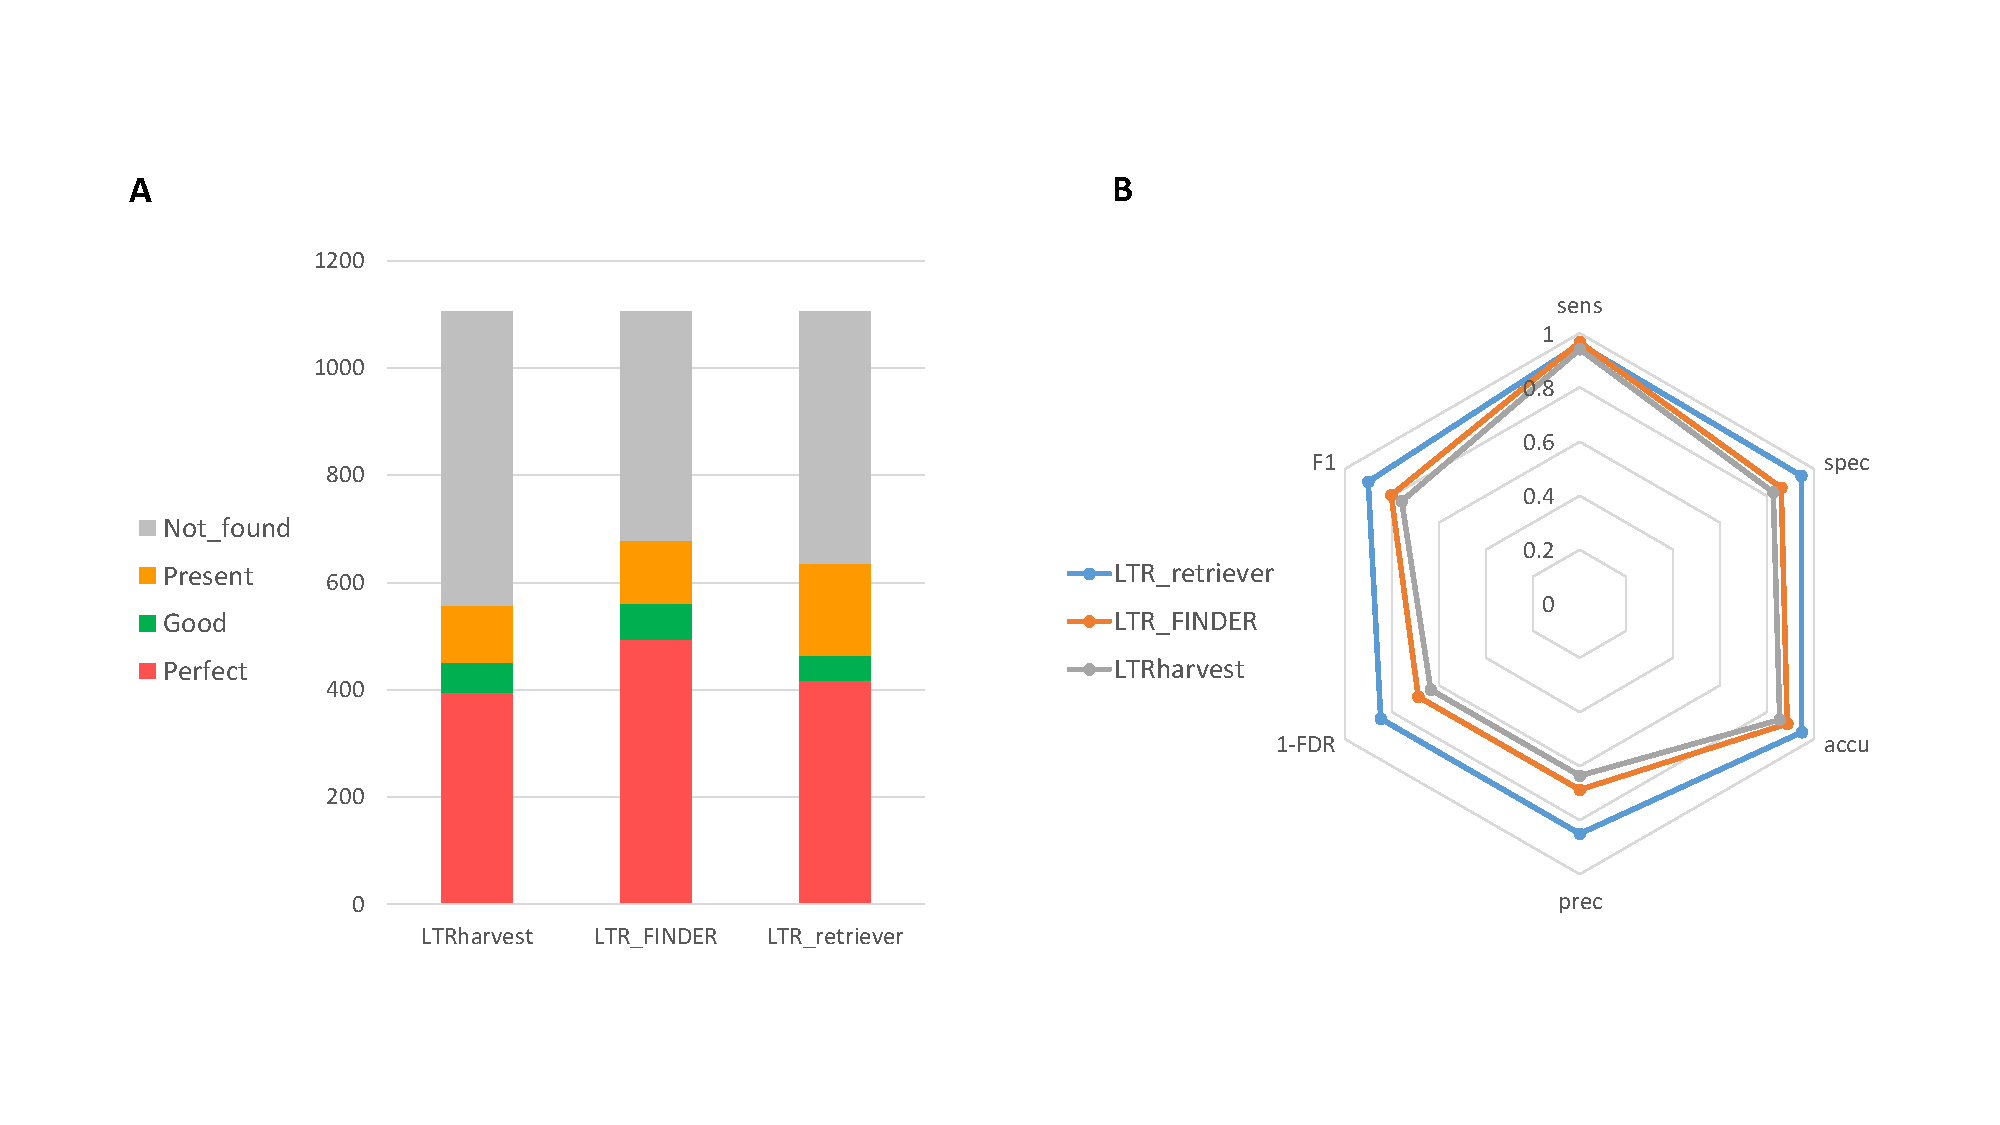
\includegraphics[width=1.0\textwidth]{figures/LTRResults.pdf}}
	\caption{Performance of LTR annotators. A the performance based on benckmarking method of RepeatModeler2 and B the performance based on benckmarking method of EDTA.}
	\label{fig:ltr_results}
\end{figure}


\subsection*{Comparison of Non-LTR annotators}
Non-LTR retrotransposons include two types of TE: LINEs and SINEs\cite{zhao2016makes}. LINEs, which lack LTRs flanking both ends, can reach several kilobases in length. Although the presence of RT and nuclease in the pol ORF of LINEs seems to provide a confident basis for their identification, there is not a database dedicated to their curation. Worsely, the truncated 5’ ends, resulting from the premature termination of reverse transcription, make them difficult to discover. SINEs, on the other hand, are much shorter (80–500 bp)\cite{wicker2007unified}. They do not encode any reverse transcriptase protein and rely on other TEs to transition, especially LINEs\cite{dewannieux2003line}. The weak signals of non-LTR retrotransposons make them quite challenging to identify\cite{mao2017sine_scan}.

To accurately identify non-LTR retrotransposons, we have developed a homology-based TE searching module, named HiTE-Non-LTR. HiTE-Non-LTR extracts LINEs and SINES consensus sequences from the Dfam library to form a non-LTR library, which is then used to search for confident candidate sequences based on the coast boundary TE candidates output by the FMEA algorithm. To benchmark the performance of the homology-based TE searching module, we use the non-LTR library to search confident candidates in the assembly based on the same parameter as the competing evaluation, called Assembly-Non-LTR. Although HiTE-Non-LTR sacrificed a little sensitivity, it achieved nearly 100\% precision.


\begin{figure}[h!]
	\centerline{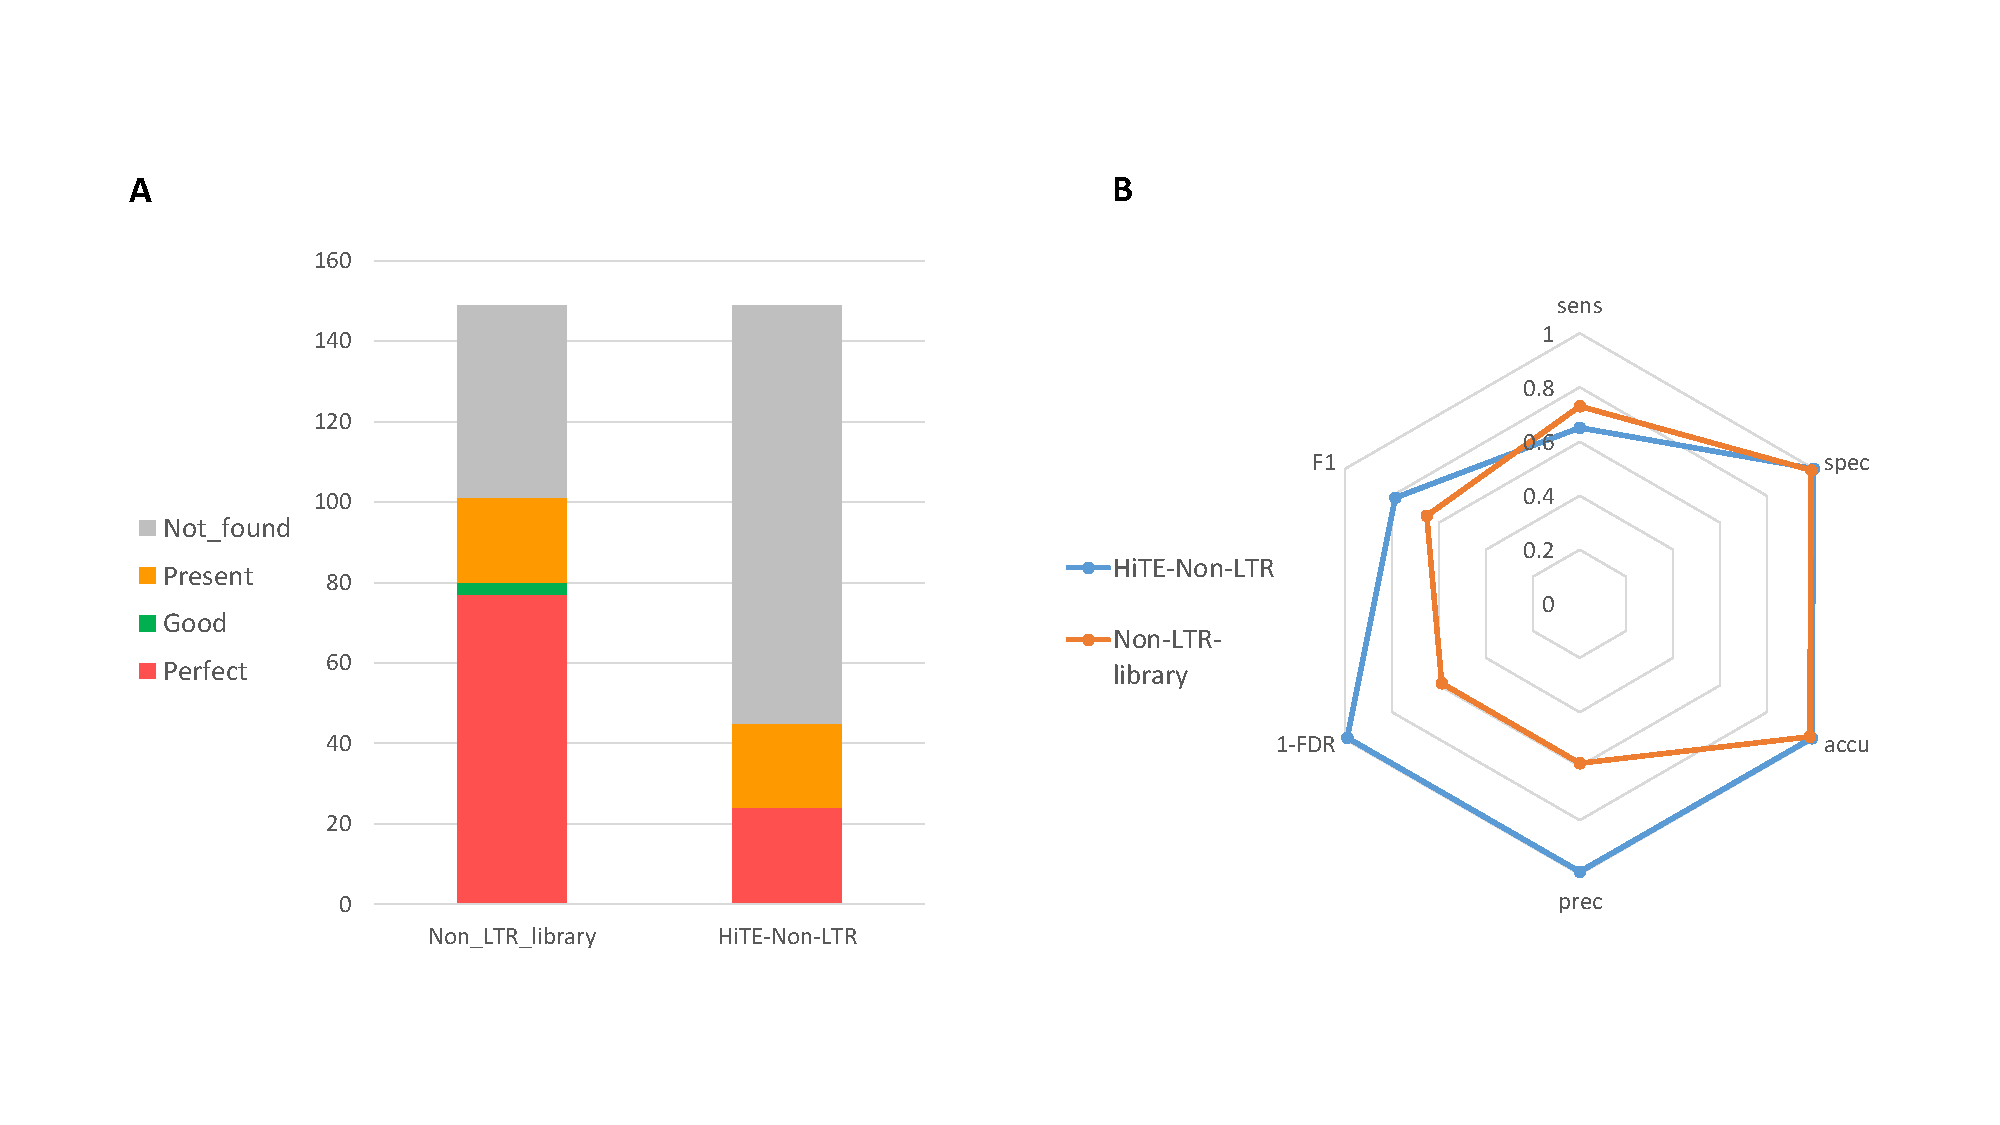
\includegraphics[width=1.0\textwidth]{figures/NonLTRResults.pdf}}
	\caption{Performance of Non-LTR annotators. A the performance based on benckmarking method of RepeatModeler2 and B the performance based on benckmarking method of EDTA.}
	\label{fig:non_ltr_results}
\end{figure}


\subsection*{Influence of parameter changes on results}
To understand how the parameters in HiTE affect the results, we selected the four most important parameters for testing: k\_num, freq\_threshold, chunk\_size, and flanking\_len. The k\_num is the size of k-mer, the freq\_threshold refers to the frequency threshold of k-mer, the chunk\_size refers to cutting the genome into blocks of the same size, and the flanking\_len is used to extend the candidate TEs identified by FMEA to search the valid TSD. These parameters have no effect on the results of LTR elements, which are discovered by LTR\_retriever. Therefore, we chose C. briggsae as the test species, whose genome only contains a small number of LTR elements.

As shown in Fig. \ref{fig:param_results}A, the smallest k\_num (such as 11) will mark the most parts of the genome as repeat regions, which cannot effectively distinguish TE from non-TE, resulting in low sensitivity and precision. Large k\_num will lose part of the true TE (lower sensitivity), but the sequences it identifies are more likely to be true TE (higher precision). Moderate k\_num (such as 31) achieves a balance between sensitivity and precision, the highest F1 value. When k\_num exceeds 41, we observe a significant drop in the number of perfect models. 
As shown in Fig. \ref{fig:param_results}B, with the freq\_threshold increased, all metrics except precision decreased significantly, which indicates that the higher the frequency of k-mer in the sequence, the more likely the sequence is to be a real TE.
As shown in Fig. \ref{fig:param_results}C, genome slicing will result in the loss of some low copy and scattered TE, reducing the sensitivity of the results significantly. The smaller the cut, the more TE will be lost.
As shown in Fig. \ref{fig:param_results}D, when flanking\_len is set to 0, the number of sensitivities and perfect models is very low, which indicates that most of the TE we identify in the FMEA algorithm have coarse boundaries. The real boundary of most TE can already be included when flanking\_len is set to 10, indicating that the error between the rough boundary in FMEA and the real boundary is not large. The metrics tend to be stable after flanking\_len is set to 40.


\begin{figure}[h!]
	\centerline{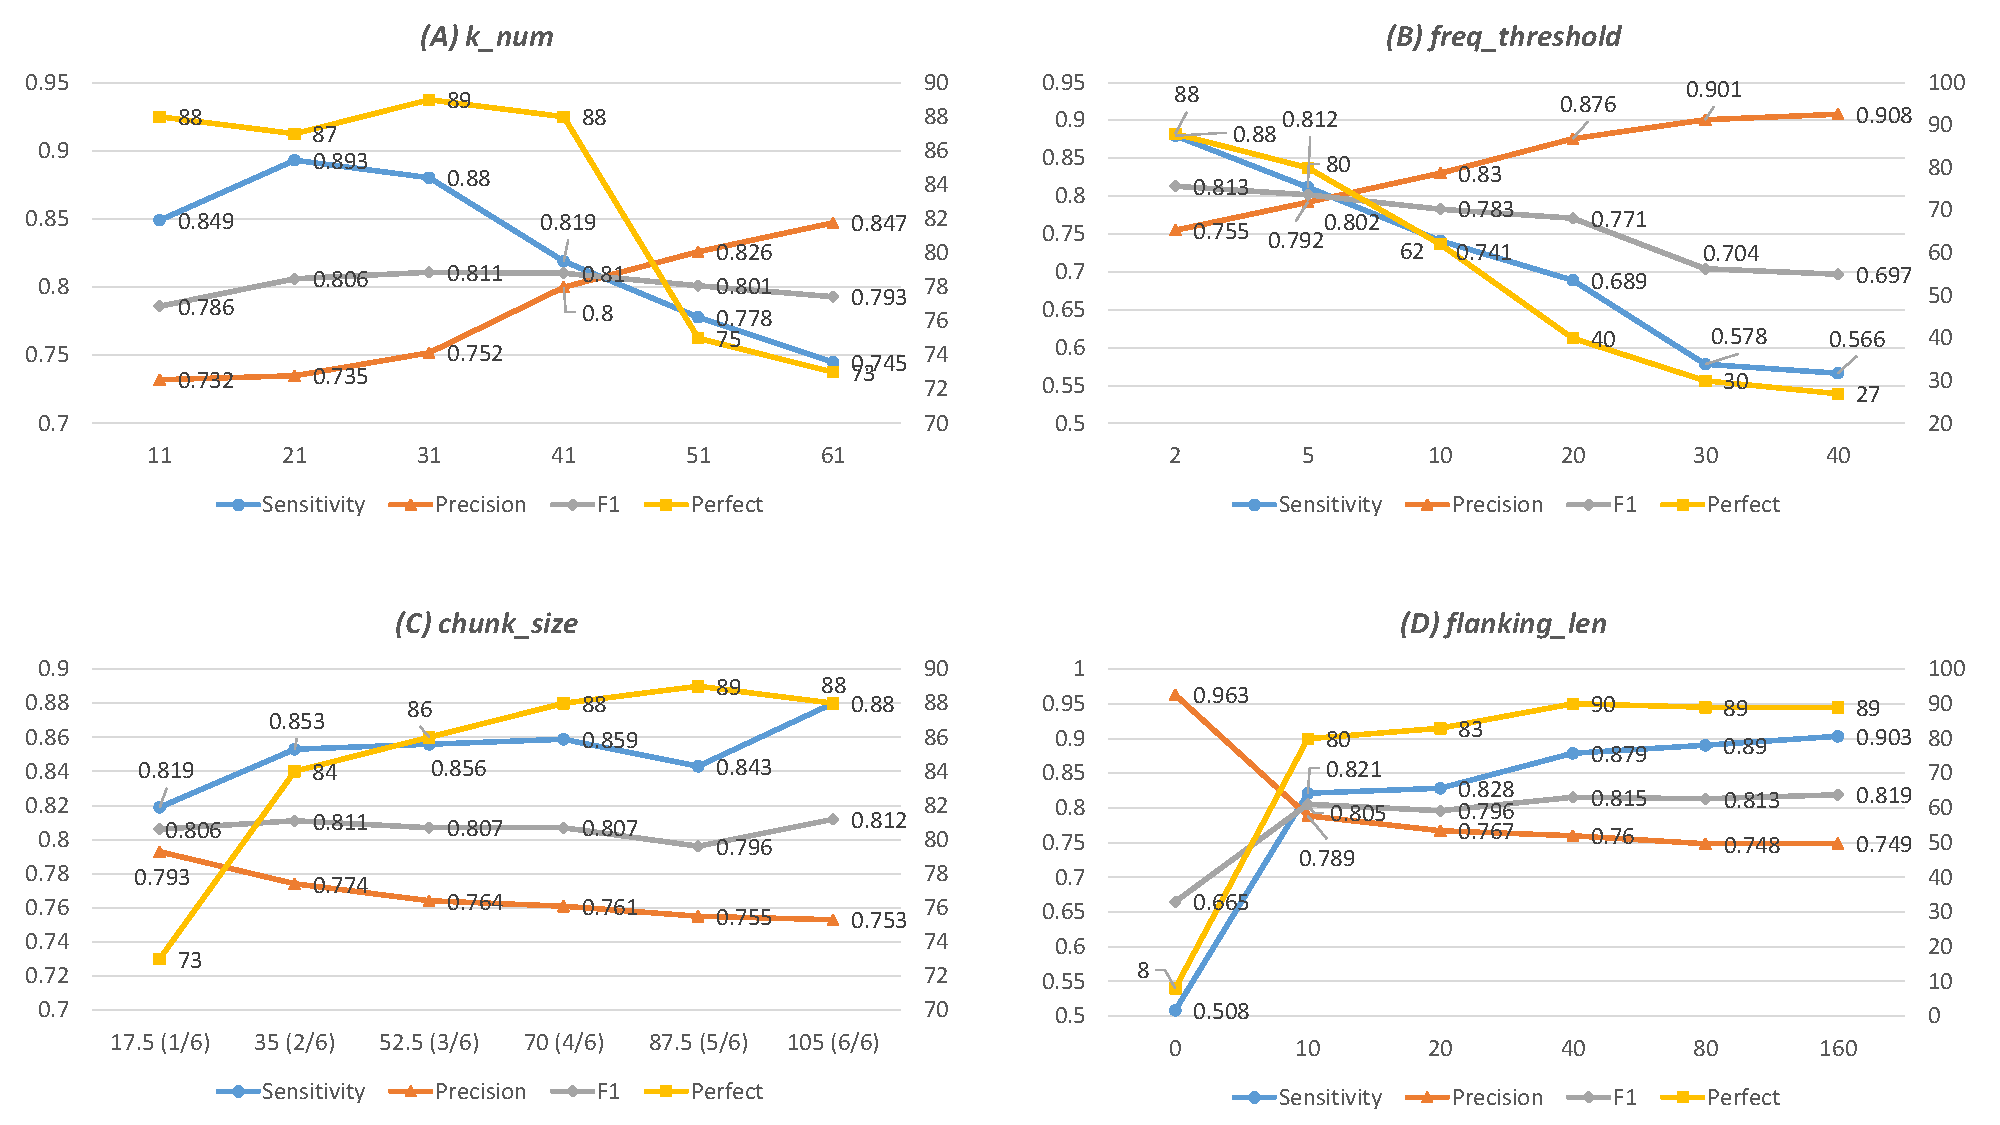
\includegraphics[width=1.0\textwidth]{figures/ParamResults.pdf}}
	\caption{Influence of parameter changes on results. A influence of k\_num parameter on results; B influence of freq\_threshold parameter on results; C influence of chunk\_size parameter on results; and D influence of flanking\_len parameter on results.}
	\label{fig:param_results}
\end{figure}

\subsection*{Contribution of TEs to genome size}

\begin{figure}[h!]
	\centerline{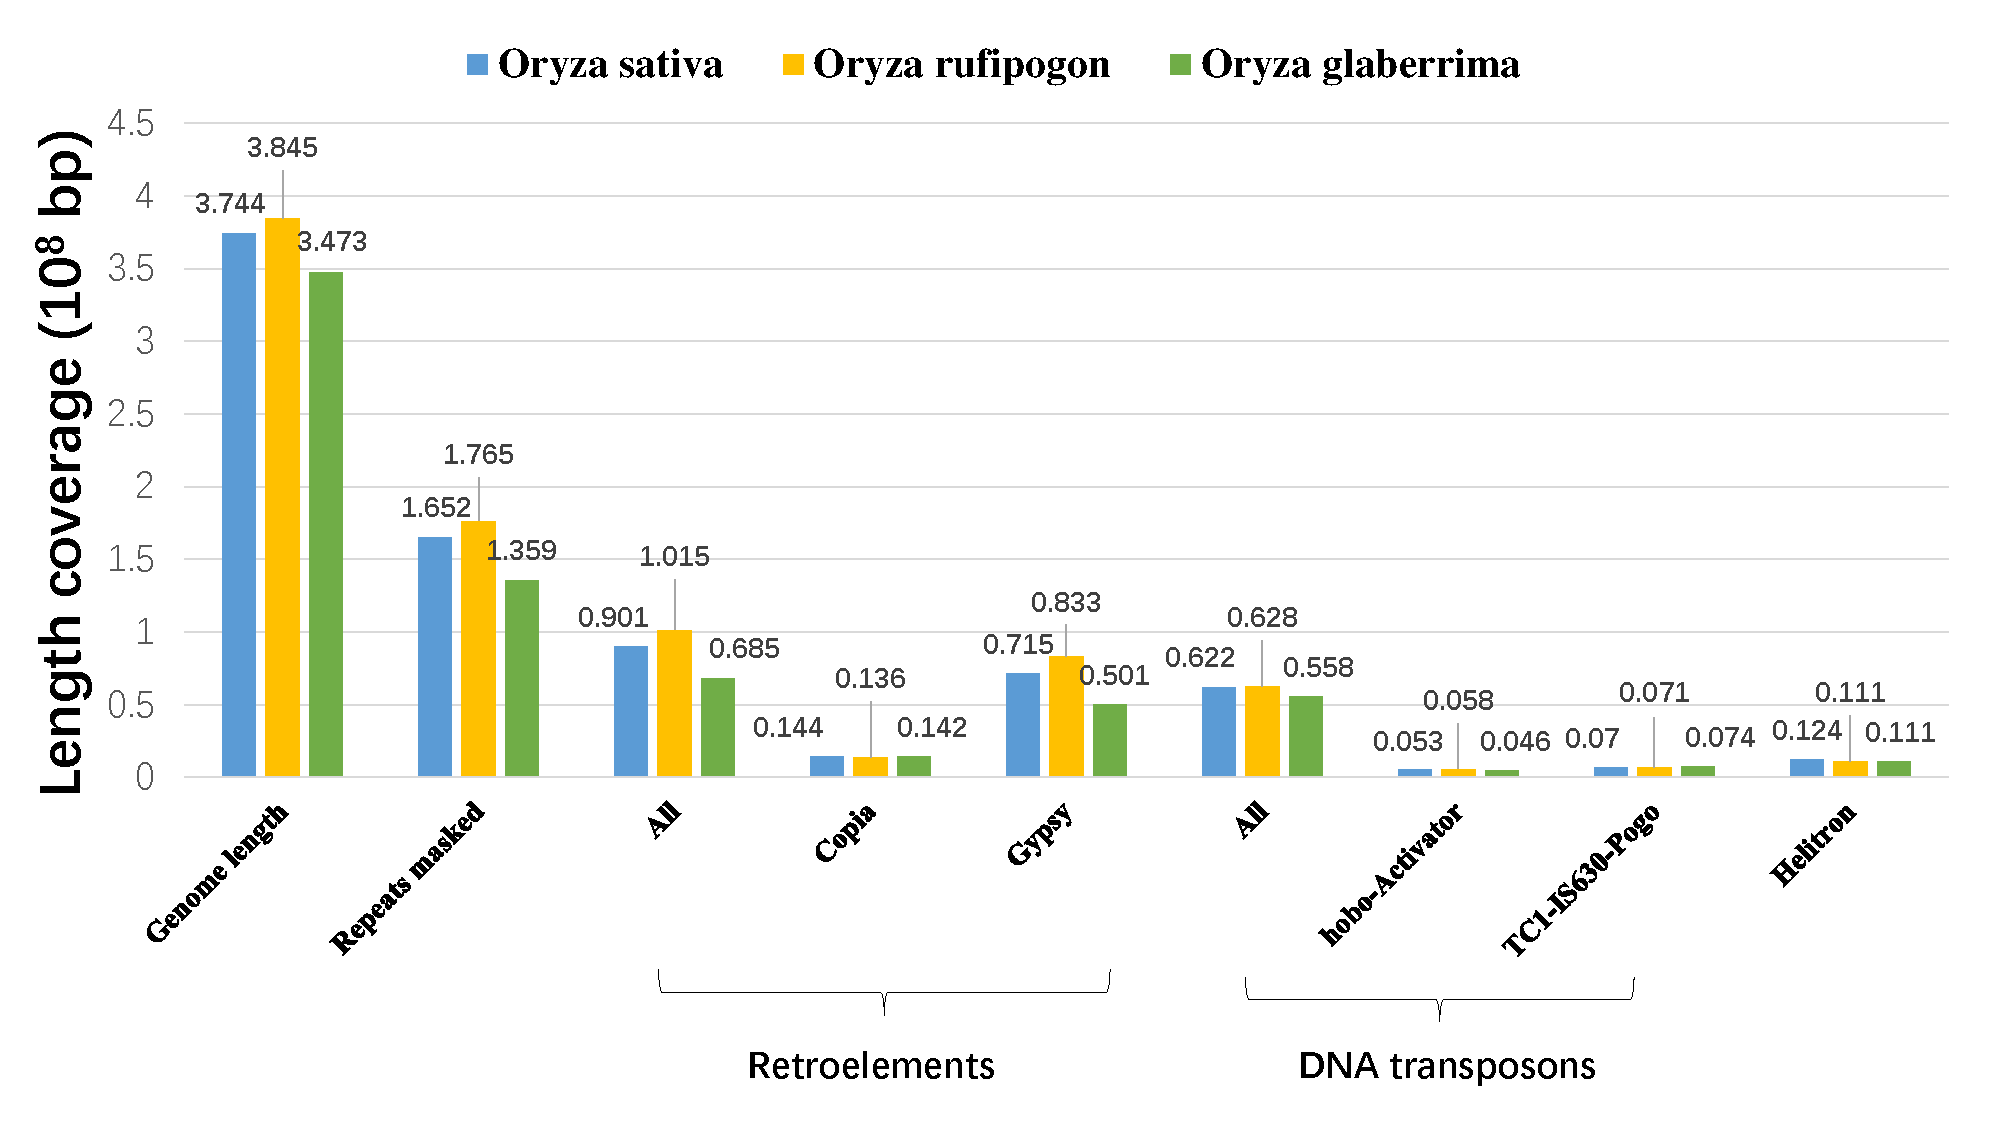
\includegraphics[width=1.0\textwidth]{figures/RiceDiff.pdf}}
	\caption{The length coverage distribution of different types of transposons based on the analysis of rice genus.}
	\label{fig:rice_diff}
\end{figure}


\section*{Discussion}
Thanks to decades of manual annotation results, we have obtained a highly reliable TE library for a limited number of species. With the development of third-generation (long-read) sequencing technology, repetitive regions in the genome can be crossed, greatly improving the quality of genome assembly. While quantities of high-quality genome assemblies are being generated, an automated and high-precision TE annotation tool is urgently needed for these newly assembled genomes. To solve this problem, we have developed an ensemble method for high-precision transposable element annotation, known as HiTE, which has performed extensive benchmarking on four model species and achieved higher metrics and restored more perfect gold standard sequences compared with other tools.

The identification of TEs requires intensive and sensitive sequence alignments, which is a computationally demanding task. HiTE uses k-mer coverage to reduce computation. Unlike the traditional k-mer-based seed expansion method, RepeatScout, HiTE uses low-frequency k-mer to determine candidate repeat areas, which reduces the number of sequence alignments and speeds up subsequent computation. 

The TE-derived sequences in the genome accumulate variations over time, making their discovery and characterization challenging for the TE annotation methods. As time goes by, TEs are often accompanied by a large number of deletion and insertion variations when replicating and copying themselves. At the same time, their insertion sites on the genome are usually random, leading to complex sequence patterns of TE in the genome, such as nested TE structures, making accurate TE identification and annotation extremely difficult. It is easy for a complete TE sequence to generate multi-segment alignment due to the influence of divergence and nested TE during its evolution. The pairwise alignment-based identification methods, such as RECON, may identify a complete TE model as multiple pieces without edges connected and generate multiple TE models using the single linkage clustering algorithm. We have designed an alignment expansion method with fault tolerance that can easily cross the large gaps caused by insertion, deletion, and nested TE and retain the complete TE structure as much as possible.

Although it is important to accurately identify the structures and boundaries of TEs, repeatedness-based methods, such as RepeatModeler\cite{Smit2008repeatmodeler}, always obtain uncertain boundaries, and intensive manual repairs are required to enable them to be saved in the cured library\cite{storer2022methodologies}. HiTE first used the sensitive sequence alignment information to determine the coarse boundaries of TEs based on the fault-tolerant alignment expansion method. Then, the coarse boundaries are flanked to search for valid TSD and terminal motifs. Finally, a reliable false-positive filtering method is developed to get confident TEs with multiple intact copies and clear TE boundaries.

Although HiTE can achieve high-precision TE identification and annotation, we do observe some losses of real TIR TEs, which are mainly caused by the following reasons:
(i) Repbase contains a large number of single-copy sequences, even zero-copy sequences. To ensure the high reliability of identified transposons, we filtered single-copy TEs, which require high homology with known transposons or TE proteins to identify. For zero-copy sequences, it is possible that these sequences come from multiple genomes of the same species, such as different types of rice, which we cannot identify based on a single genome, or they are from degraded nested TE, and there are no other full-length copies of these sequences in the genome. Our method needs at least two full-length copies to determine whether a sequence is a true transposon, so we have left out most of the single-copy and zero-copy sequences.
(ii) Some transposons do not have consistent TSD or even any TSD. To achieve high-precision identification, we identify LTR and TIR TEs by TSD, so those TEs that do not have consistent TSD are filtered out. Highly divergent terminal inverted sequences (identity less than 0.7) and the candidate TEs with accidental sequence homology outside the boundary, which is similar to many false positive patterns, are also filtered out. We discover some lost real TIRs by manually reviewing FMEA results. These TIRs are filtered out for various reasons, such as the lack of a consistent TSD and the big divergence in the first 5-bp of the TIRs. This further proves the effectiveness of the FMEA method. At the same time, a more accurate and comprehensive filtering method helps to find more real TIRs.

We found that the identification of TEs with weak structural characteristics, such as Helitron and non-LTR elements, is very challenging. Although we have greatly improved the identification performance of Helitron, there is still potential for improvement. For example, a more comprehensive hairpin loop pattern will significantly improve the sensitivity.

To date, due to the truncated 5' ends of LINEs, there is no method to identify LINEs based on the structure method. A few tools designed for identification of SINEs, which suffer from the high false positives and low sensitivity. To achieve high-precision non-LTR element annotation, we developed a homology-based TE searching method, which improves precision by nearly 100\%. However, we do lose some true non-LTR elements, and the structure-based identification methods of LINEs are needed, which is also the direction of our future efforts.


\section*{Conclusions}
The rapid development of sequencing technology enables us to obtain a more reliable genome assembly. The TE library generated by an inaccurate TE identification tool will contain many errors, which will be propagated during the whole-genome annotation process. HiTE makes full use of the strengths and weaknesses of existing methods, including ensemble methods of many types, and can comprehensively and accurately identify and annotate TEs in assembly. By benchmarking on four model species with different TE landscapes, we prove that HiTE can achieve higher accuracy and restore more perfect gold standard TE models, which can be fully applied to any new sequencing genome assembly.

\section*{Methods}
Text and results for this section, as per the individual journal's instructions for authors.

In this section we examine the growth rate of the mean of $Z_0$, $Z_1$ and $Z_2$. In
addition, we examine a common modeling assumption and note the
importance of considering the tails of the extinction time $T_x$ in
studies of escape dynamics.
We will first consider the expected resistant population at $vT_x$ for
some $v>0$, (and temporarily assume $\alpha=0$)
%
\[
E \bigl[Z_1(vT_x) \bigr]=
\int_0^{v\wedge
1}Z_0(uT_x)
\exp (\lambda_1)\,du .
\]
%
If we assume that sensitive cells follow a deterministic decay
$Z_0(t)=xe^{\lambda_0 t}$ and approximate their extinction time as
$T_x\approx-\frac{1}{\lambda_0}\log x$, then we can heuristically
estimate the expected value as
%
\begin{equation}\label{eqexpmuts}
\begin{aligned}[b]
&      E\bigl[Z_1(vT_x)\bigr]\\
&\quad      = \frac{\mu}{r}\log x
\int_0^{v\wedge1}x^{1-u}x^{({\lambda_1}/{r})(v-u)}\,du .
\end{aligned}
\end{equation}
%


\section*{Supplementary information}
Supplementary information accompanies this paper at

%%%%%%%%%%%%%%%%%%%%%%%%%%%%%%%%%%%%%%%%%%%%%%
%%                                          %%
%% Backmatter begins here                   %%
%%                                          %%
%%%%%%%%%%%%%%%%%%%%%%%%%%%%%%%%%%%%%%%%%%%%%%

\begin{backmatter}

\section*{Acknowledgements}%% if any
This work was carried out in part using computing resources at the High Performance Computing Center of Central South University.

\section*{Funding}%% if any
This work has been supported by the National Natural Science Foundation of China under Grant: No.61772557 and No.62002388, Hunan Provincial Science and technology Program (No.2018wk4001), 111 Project (No.B18059), Fundamental Research Funds for the Central Universities of Central South University (2021zzts0208).

\section*{Abbreviations}%% if any
Text for this section\ldots

\section*{Availability of data and materials}%% if any
Text for this section\ldots

\section*{Ethics approval and consent to participate}%% if any
Not applicable.

\section*{Competing interests}
The authors declare that they have no competing interests.

\section*{Consent for publication}%% if any
Not applicable.

\section*{Authors' contributions}
Text for this section \ldots

\section*{Authors' information}%% if any
Text for this section\ldots

%%%%%%%%%%%%%%%%%%%%%%%%%%%%%%%%%%%%%%%%%%%%%%%%%%%%%%%%%%%%%
%%                  The Bibliography                       %%
%%                                                         %%
%%  Bmc_mathpys.bst  will be used to                       %%
%%  create a .BBL file for submission.                     %%
%%  After submission of the .TEX file,                     %%
%%  you will be prompted to submit your .BBL file.         %%
%%                                                         %%
%%                                                         %%
%%  Note that the displayed Bibliography will not          %%
%%  necessarily be rendered by Latex exactly as specified  %%
%%  in the online Instructions for Authors.                %%
%%                                                         %%
%%%%%%%%%%%%%%%%%%%%%%%%%%%%%%%%%%%%%%%%%%%%%%%%%%%%%%%%%%%%%

% if your bibliography is in bibtex format, use those commands:
\bibliographystyle{bmc-mathphys} % Style BST file (bmc-mathphys, vancouver, spbasic).
\bibliography{bmc_article}      % Bibliography file (usually '*.bib' )
% for author-year bibliography (bmc-mathphys or spbasic)
% a) write to bib file (bmc-mathphys only)
% @settings{label, options="nameyear"}
% b) uncomment next line
%\nocite{label}

% or include bibliography directly:
% \begin{thebibliography}
% \bibitem{b1}
% \end{thebibliography}

%%%%%%%%%%%%%%%%%%%%%%%%%%%%%%%%%%%
%%                               %%
%% Figures                       %%
%%                               %%
%% NB: this is for captions and  %%
%% Titles. All graphics must be  %%
%% submitted separately and NOT  %%
%% included in the Tex document  %%
%%                               %%
%%%%%%%%%%%%%%%%%%%%%%%%%%%%%%%%%%%

%%
%% Do not use \listoffigures as most will included as separate files

\section*{Figures}
  \begin{figure}[h!]
  \caption{Sample figure title}
\end{figure}

\begin{figure}[h!]
  \caption{Sample figure title}
\end{figure}

%%%%%%%%%%%%%%%%%%%%%%%%%%%%%%%%%%%
%%                               %%
%% Tables                        %%
%%                               %%
%%%%%%%%%%%%%%%%%%%%%%%%%%%%%%%%%%%

%% Use of \listoftables is discouraged.
%%
\section*{Tables}
\begin{table}[h!]
\caption{Sample table title. This is where the description of the table should go}
  \begin{tabular}{cccc}
    \hline
    & B1  &B2   & B3\\ \hline
    A1 & 0.1 & 0.2 & 0.3\\
    A2 & ... & ..  & .\\
    A3 & ..  & .   & .\\ \hline
  \end{tabular}
\end{table}

%%%%%%%%%%%%%%%%%%%%%%%%%%%%%%%%%%%
%%                               %%
%% Additional Files              %%
%%                               %%
%%%%%%%%%%%%%%%%%%%%%%%%%%%%%%%%%%%

\section*{Additional Files}
  \subsection*{Additional file 1 --- Sample additional file title}
    Additional file descriptions text (including details of how to
    view the file, if it is in a non-standard format or the file extension).  This might
    refer to a multi-page table or a figure.

  \subsection*{Additional file 2 --- Sample additional file title}
    Additional file descriptions text.

\end{backmatter}
\end{document}
